%%%%%%%%%%%%%%%%%%%%%%%%%%%%%%%%%%%%%%%%%
% Beamer Presentation
% LaTeX Template
% Version 1.0 (10/11/12)
%
% This template has been downloaded from:
% http://www.LaTeXTemplates.com
%
% License:
% CC BY-NC-SA 3.0 (http://creativecommons.org/licenses/by-nc-sa/3.0/)
%
%%%%%%%%%%%%%%%%%%%%%%%%%%%%%%%%%%%%%%%%%

%----------------------------------------------------------------------------------------
%	PACKAGES AND THEMES
%----------------------------------------------------------------------------------------
\documentclass[xcolor=table]{beamer}
\mode<presentation> {
	
	% The Beamer class comes with a number of default slide themes
	% which change the colors and layouts of slides. Below this is a list
	% of all the themes, uncomment each in turn to see what they look like.
	
	%\usetheme{default}
	%\usetheme{AnnArbor}
	%\usetheme{Antibes}
	%\usetheme{Bergen}
	%\usetheme{Berkeley}
	%\usetheme{Berlin}
	%\usetheme{Boadilla}
	%\usetheme{CambridgeUS}
	%\usetheme{Copenhagen} % molto vicino a come lo voglio%
	%\usetheme{Darmstadt}
	%\usetheme{Dresden}
	%\usetheme{Frankfurt}
	%\usetheme{Goettingen}
    %\usetheme{Hannover} % non così male%
	%\usetheme{Ilmenau}
	%\usetheme{JuanLesPins}
	%\usetheme{Luebeck}
	\usetheme{Madrid}
	%\usetheme{Malmoe}
	%\usetheme{Marburg}
	%\usetheme{Montpellier}
	%\usetheme{PaloAlto}
	%\usetheme{Pittsburgh}
	%\usetheme{Rochester}
	%\usetheme{Singapore}
	%\usetheme{Szeged}
	%\usetheme{Warsaw}
	
	% As well as themes, the Beamer class has a number of color themes
	% for any slide theme. Uncomment each of these in turn to see how it
	% changes the colors of your current slide theme.
	
	%\usecolortheme{albatross}
	%\usecolortheme{beaver} %standard%
	%\usecolortheme{beetle}
	%\usecolortheme{crane}
	%\usecolortheme{dolphin} %non male%
	%\usecolortheme{dove}
	%\usecolortheme{fly}
	%\usecolortheme{lily}
	%\usecolortheme{orchid} 
	%\usecolortheme{rose} %buono!%
	%\usecolortheme{seagull}
	%\usecolortheme{seahorse}
	\usecolortheme{whale}
	%\usecolortheme{wolverine}
	
	%\setbeamertemplate{footline} % To remove the footer line in all slides uncomment this line
	%\setbeamertemplate{footline}[page number] % To replace the footer line in all slides with a simple slide count uncomment this line
	
	%\setbeamertemplate{navigation symbols}{} % To remove the navigation symbols from the bottom of all slides uncomment this line
}

\usepackage{graphicx} % Allows including images
\usepackage{booktabs} % Allows the use of \toprule, \midrule and \bottomrule in tables
\usepackage[latin1]{inputenc}
\usepackage{floatflt,epsfig}
\usepackage{color}
\usepackage{tabto}
\usepackage{verbatim}
\usepackage{movie15}
\usepackage{amsmath}
\usepackage{mathtools}
\usepackage{lipsum}
\usepackage{setspace}
\DeclarePairedDelimiter{\abs}{\lvert}{\rvert}
%----------------------------------------------------------------------------------------
%	TITLE PAGE
%----------------------------------------------------------------------------------------

\title[Introduction to research activities]{Introduction to research activities exam} % The short title appears at the bottom of every slide, the full title is only on the title page
\author{Student: Arianna Mischianti} % Your name
\institute[] % Your institution as it will appear on the bottom of every slide, may be shorthand to save space
{Supervisors: \\
\emph{Prof.} G. Mistura \\ 
\emph{Dott.} P. Sartori \\% Your institution for the title page
\medskip 
\textit{University of Padova} % Your email address
}
\date{Padova, Luglio 2020} % Date, can be changed to a custom date

\begin{document}

%%%%%%%%%%%%%%%%%%%%%%%%%%%%%%%%%%%%%%%%%%%%%%%%%%%%%%%%%%%%%%%%%%%%%%%%%%
	
	\begin{frame}
	\centering \titlepage 
\end{frame}

%%%%%%%%%%%%%%%%%%%%%%%%%%%%%%%%%%%%%%%%%%%%%%%%%%%%%%%%%%%%%%%%%%%%%%%%%%
\begin{frame}
\frametitle{Abstract} 
\fontsize{11}{12.2} \selectfont
\begin{columns}
	\begin{column}{.4\textwidth}
		Title of the experience: \textbf{Rheological measurements of non-newtonian liquids based on drop oscillation.}\\
		\medskip
		\fontsize{10}{12.2} \selectfont
		This research activity deals with the reproduction of a rheometer  by means of an implemented \textit{ad hoc} experimental apparatus to study vibrational normal modes of submillimetric sessile drops (volumes of $pL/\mu L$), from which it is possible to estimate \textbf{viscosity} and \textbf{surface tension}.\\
\end{column}
\begin{column}{.6\textwidth}
\centering
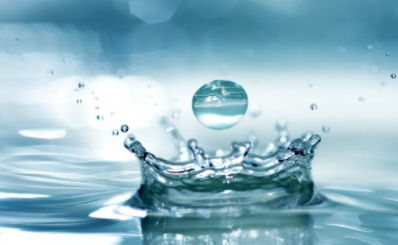
\includegraphics[width=0.35\columnwidth]{acqua.PNG}
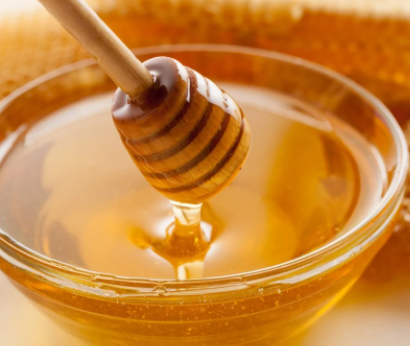
\includegraphics[width=0.35\columnwidth]{miele.PNG}\\
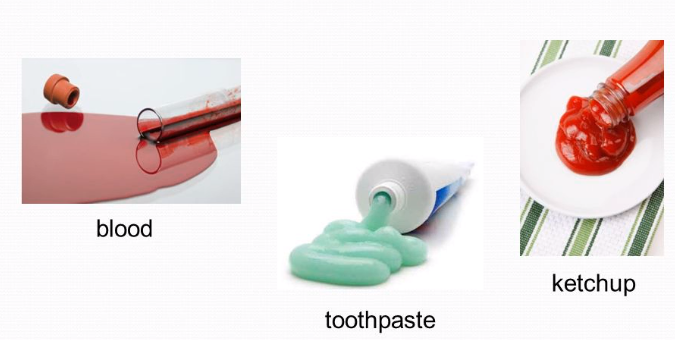
\includegraphics[width=0.7\columnwidth]{nonnewtesempi.PNG}\\
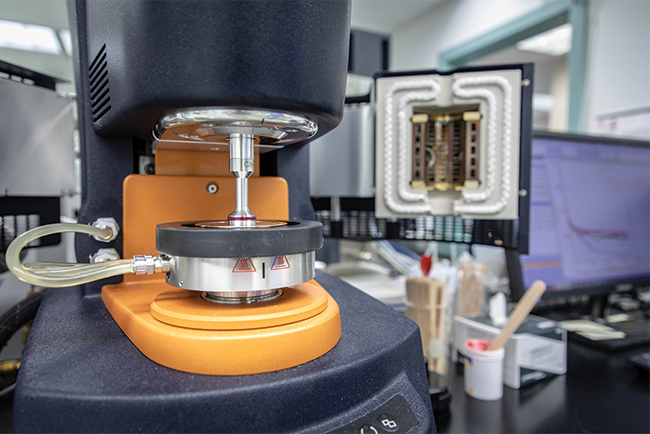
\includegraphics[width=0.7\columnwidth]{rheometer_full_width.jpg}\\
\end{column}
\end{columns}
\end{frame}

%%%%%%%%%%%%%%%%%%%%%%%%%%%%%%%%%%%%%%%%%%%%%%%%%%%%%%%%%%%%%%%%%%%%%%%%%%%
\begin{frame}
\frametitle{Principle of the experiment} 
\fontsize{11}{12.2} \selectfont
\begin{columns}
	\begin{column}{.5\textwidth}
		\centering
		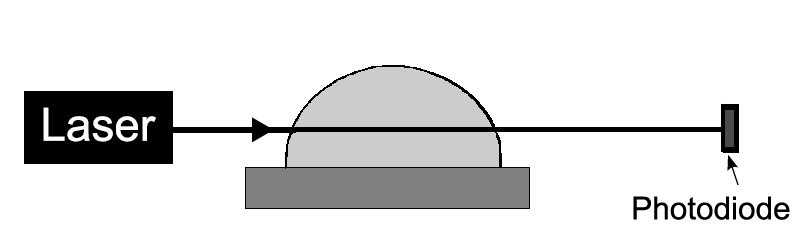
\includegraphics[width=0.8\columnwidth]{introduzione1.PNG}\\
		$\big\Downarrow$\\
		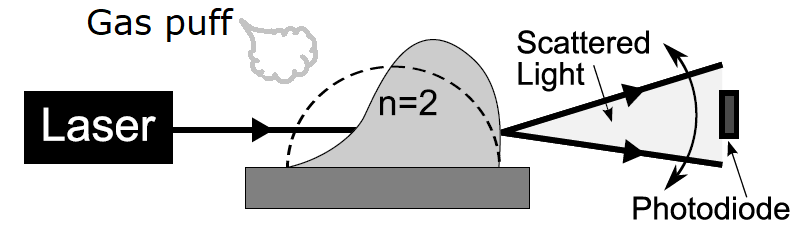
\includegraphics[width=0.8\columnwidth]{introduzione.PNG}\\
		$\big\Downarrow$\centering\\
		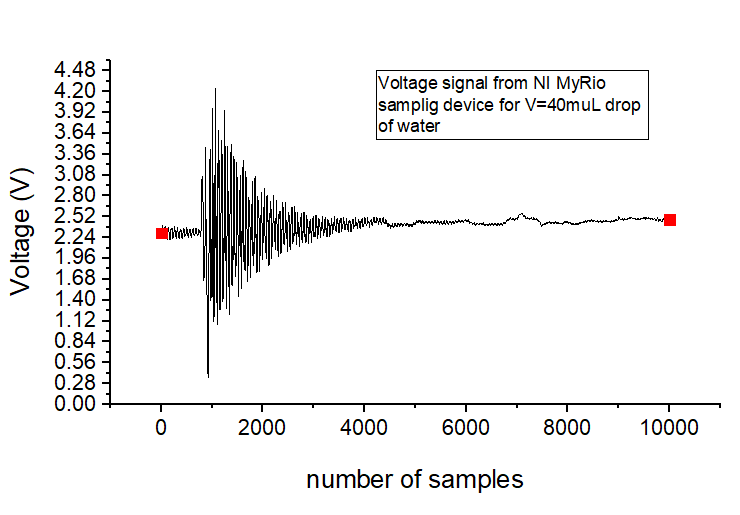
\includegraphics[width=0.8\columnwidth]{voltagesignal.PNG}\\
	\end{column}
	\begin{column}{.7\textwidth}
		$\nearrow$ 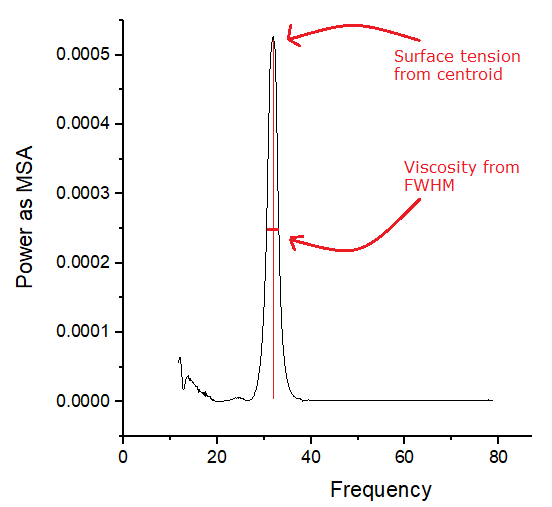
\includegraphics[width=0.7\columnwidth]{picco_f_fwhm.png}\\
		
	\end{column}
\end{columns}

\end{frame}
%%%%%%%%%%%%%%%%%%%%%%%%%%%%%%%%%%%%%%%%%%%%%%%%%%%%%%%%%%%%%%%%%%%%%
%%%%%%%%%%%%%%%%%%%%%%%%%%%%%%%%%%%%%%%%%%%%%%%%%%%%%%%%%%%%%%%%%%%%%%%%%%%
\begin{frame}

\frametitle{Aim of the experience}
\fontsize{11}{13.2} \selectfont

\begin{columns}
	\begin{column}{.45\textwidth}
		\begin{itemize}
			\item	To reproduce a \textbf{Rheometer}
			\item	To find the resonance spectra
			\item	To compute surface tension and viscosity
			\item	To repeat the process for \textbf{Newtonian} liquids: water and glycerine solutions: 60\%,75\%,85\%.
		\end{itemize}
		
		
	\end{column}
	\begin{column}{.45\textwidth}
		\centering
		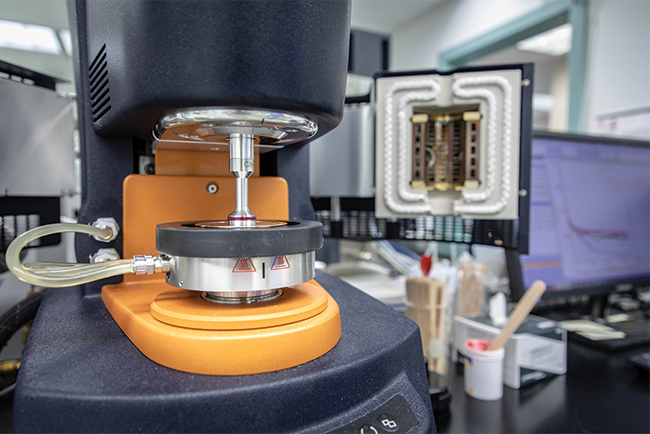
\includegraphics[width=.8\columnwidth]{rheometer_full_width.jpg}\\	
		\medskip
		$\big\Downarrow$\\
		\medskip
		\centering
		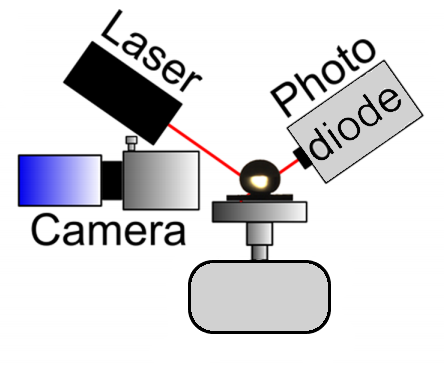
\includegraphics[width=.8\columnwidth]{setup.png}
	\end{column}
\end{columns}

\end{frame}

%%%%%%%%%%%%%%%%%%%%%%%%%%%%%%%%%%%%%%%%%%%%%%%%%%%%%%%%%%%%%%%%%%%

\begin{frame}

\frametitle{Basic theory - Viscosity}
\fontsize{10}{13.2} \selectfont
The viscosity of a fluid is a measure of its resistance to deformation at a given rate.
\begin{columns}
	\begin{column}{.5\textwidth}
		Shear Rate:
		\begin{equation*}
		\dot{\gamma}=\frac{\partial v}{\partial z}
		\end{equation*}
	\end{column}
	\begin{column}{.5\textwidth}
		Shear stress:
		\begin{equation*}
		\tau=\frac{F}{S}
		\end{equation*}
	\end{column}
\end{columns}
\medskip

The constant of proportionality between the two rheological quantities is the viscosity coefficient:
\medskip
\begin{columns}
	\begin{column}{.5\textwidth}
		Newtonian Fluids:
		\begin{equation*}
		\tau=\eta\dot{\gamma}
		\end{equation*}
	\end{column}
	\begin{column}{.5\textwidth}
		Non-Newtonian Fluids:
		\begin{equation*}
		\tau=\eta(\dot{\gamma})\dot{\gamma}
		\end{equation*}
	\end{column}
\end{columns}
\centering
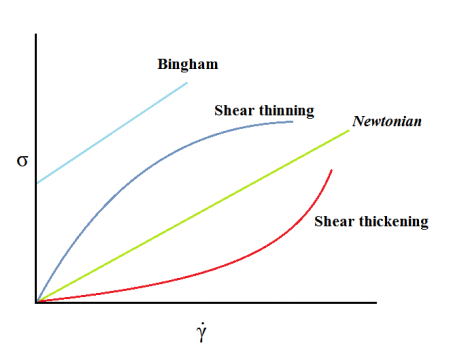
\includegraphics[width=.4\columnwidth]{Nonnewtonianieta.png}

\end{frame}
%%%%%%%%%%%%%%%%%%%%%%%%%%%%%%%%%%%%%%%%%%%%%%%%%%%%%%%%%%%%%%%%%%%%%%%%%%
\begin{frame}
\frametitle{Basic theory - Surface tension}
\fontsize{11}{0}
\bigskip
Surface tension $\sigma$ is the energy, or work, due to intermolecular forces, required to increase a unit of the surface area.
\begin{equation}
\sigma=\bigg(\frac{\partial G}{\partial A}\bigg)_{T,p}=\frac{dF}{dL}
\end{equation}
\bigskip
In \textbf{Microfluidics} capillary force dominate over gravity force
\begin{columns}
	\begin{column}{.5\textwidth}
		\centering
		\textit{Bond} Number:
		\begin{equation*}
		Bo=\frac{F_{gravity}}{F_{capillary}}=
		\end{equation*}
		\begin{equation*}
		=\frac{\rho g L^2}{\sigma}<<1.
		\end{equation*}
	\end{column}
	\begin{column}{.7\textwidth}
		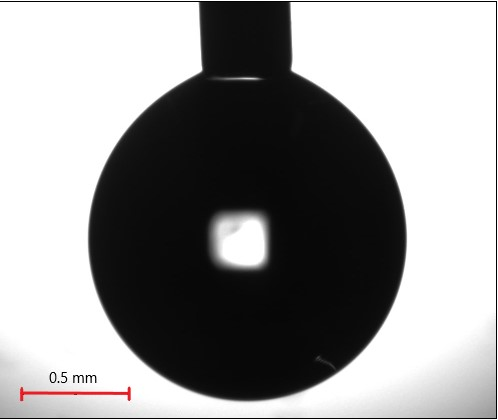
\includegraphics[width=.4\columnwidth]{prova_0019A.jpg}
		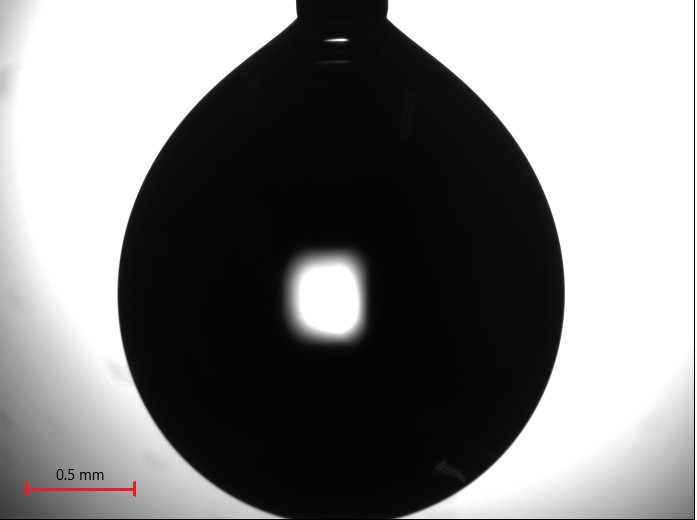
\includegraphics[width=.4\columnwidth]{prova_0115A.jpg}
	\end{column}
\end{columns}
\end{frame}


%%%%%%%%%%%%%%%%%%%%%%%%%%%%%%%%%%%%%%%%%%%%%%%%%%%%%%%%%%%%%%%%%%%%%%%%%%%
\begin{frame}

\frametitle{Surface tension and contact angle}

\fontsize{11}{13.2} \selectfont

\begin{columns}
\begin{column}{.55\textwidth}
The contact angle is the angle between the solid/liquid and the tangent  to the liquid/air interface where they meet. It quantifies the wettability of a solid surface by a liquid via the Young equation:
\begin{equation}
cos\theta_E=\frac{\sigma_{SG}-\sigma_{SL}}{\sigma}.
\end{equation}
\end{column}
\begin{column}{.3\textwidth}
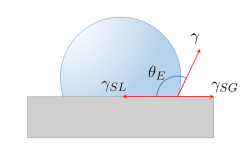
\includegraphics[width=1.2\columnwidth]{angolo.png}\\
\end{column}
\end{columns}
\end{frame}
%%%%%%%%%%%%%%%%%%%%%%%%%%%%%%%%%%%%%%%%%%%%%%%%%%%%%%%%%%%%%%%%%%%%%%%%%%%
\begin{frame}

\frametitle{wettability}
\fontsize{11}{13.2} \selectfont
\begin{columns}
\begin{column}{.4\textwidth}
 Depending on the contact angle we can define:
\begin{itemize}
	\item $\theta_E=0^\circ$ $perfect\ wettability$;
	\item $\theta_E<90^\circ$ $hydrophilic$;
	\item $\theta_E>90^\circ$ $hydrophobic$;
	\item $\theta_E>150^\circ$ $super\ hydrophobic$.
\end{itemize}
\end{column}
\begin{column}{.5\textwidth}
\begin{figure}
	\fontsize{3}{3} \selectfont
	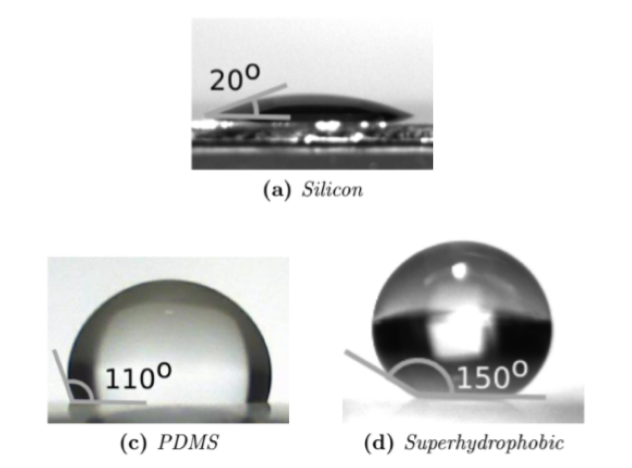
\includegraphics[width=1.1\columnwidth]{Gocce_sessili.PNG} 
\end{figure}
\end{column}
\end{columns}
\end{frame}
%%%%%%%%%%%%%%%%%%%%%%%%%%%%%%%%%%%%%%%%%%%%%%%%%%%%%%%%%%%%%%%%%%%%%%%%%%%
\begin{frame}

\frametitle{Pinning and hysteresis of contact angle}
\fontsize{11}{13.2} \selectfont
\begin{columns}
\begin{column}{.55\textwidth}
\textbf{Contact line}: three phase separator line.\\
\medskip
\textbf{hysteresis of contact angle}: is the result of the activation energy required for movement of a droplet from one metastable state to another on a surface, caused by asperity, impurities or chemical or physical disomogeneity in an interval $\theta=[\theta_R;\theta_A]$ (Reciding A. and Advancing A.).\\
\medskip
\textbf{Pinning}:when the contact line remains blocked and the contact angle undergoes a phenomenon of hysteresis.
\end{column}
\begin{column}{.25\textwidth}
		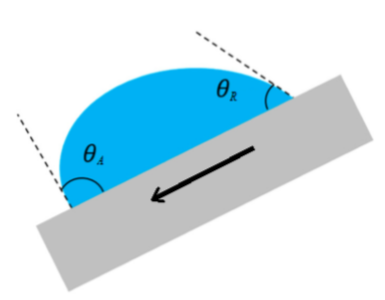
\includegraphics[width=1.3\columnwidth]{pinningg.png}
\end{column}
\end{columns}
\end{frame}


%%%%%%%%%%%%%%%%%%%%%%%%%%%%%%%%%%%%%%%%%%%%%%%%%%%%%%%%%%%%%%%%%%%%%



\begin{frame}
\frametitle{Vibrational modes of oscillating sessile droplets}
\fontsize{10}{11.2} \selectfont
\begin{columns}
	\begin{column}{.6\textwidth}
		In proposed models, a drop is seen as a \textbf{damped oscillator}. \\
		Hipotesis: Pinned contact line, hydrophobic substrate, capillary force predominate over gravity force
\end{column}
\begin{column}{.25\textwidth}
	 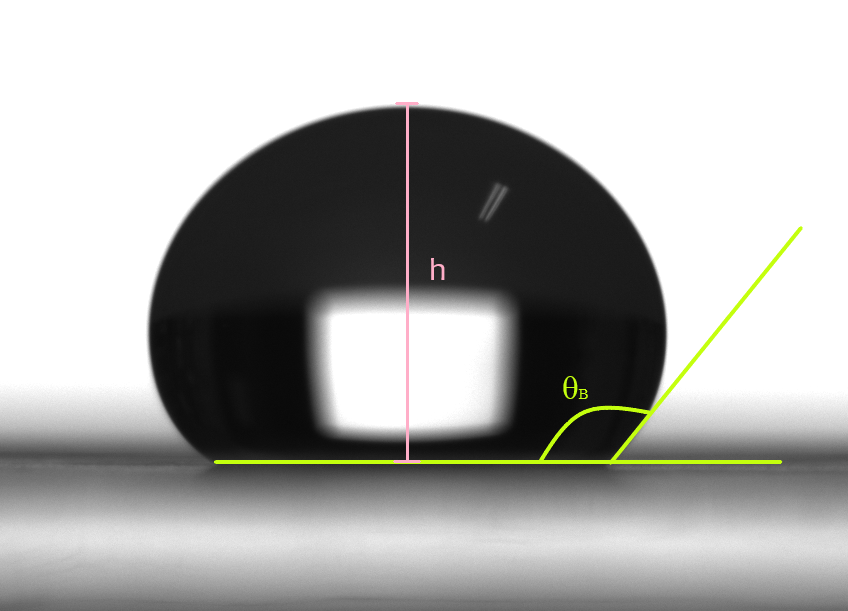
\includegraphics[width=0.9\columnwidth]{40muL_3.png}
\end{column}
\end{columns}
		\begin{itemize}
			\item \textit{Sharp et al.} - \textbf{2011} Analysis of vertical modes for droplets in capillary regime considering a spherical surface. An homogeneous factor of  $\alpha\simeq0.81$ is found to correct the formula:
		\begin{equation}
		f_n\simeq\alpha\frac{\pi}{2}\sqrt{\frac{n^3\sigma}{24\rho V}\frac{cos^3\theta-3cos\theta+2}{\theta^3}}
		\end{equation}
			\end{itemize}
			
\centering
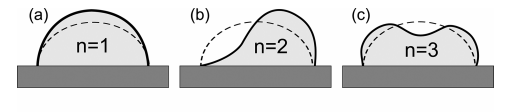
\includegraphics[width=.6\columnwidth]{modi.png}

\end{frame}
%%%%%%%%%%%%%%%%%%%%%%%%%%%%%%%%%%%%%%%%%%%%%%%%%%%%%%%%%%%%%%%%%%%%%
%%%%%%%%%%%%%%%%%%%%%%%%%%%%%%%%%%%%%%%%%%%%%%%%%%%%%%%%%%%%%%%%%%%%%%%%%%

\begin{frame}

\frametitle{ Temperton theory and Viscosity calculus}

\fontsize{10}{11.2} \selectfont
	\begin{itemize}
	\item \textit{Temperton et al.} - \textbf{2013} Improved the Sharp's formula by including a geometrical factor that represents the height of the drop:
	\begin{equation}
	f_n=\frac{1}{\pi 2}\sqrt{\frac{n^3\sigma\pi}{4\rho V}tanh\bigg[\frac{n\pi}{4\theta}\frac{-cos^4\theta+6cos^2\theta-8cos\theta+3}{cos^3\theta-3cos\theta+2}\bigg]}
	\end{equation}
\end{itemize}

\textbf{Viscosity:}

\textit{R. Temperton} - \textbf{2012} The oscillations decay exponentially with time such that the amplitude scales with $e^{-\Gamma t}$ where $\Gamma$ is the damping coefficient:
\begin{equation}
\Gamma_{bulk} = \frac{2}{\rho}\bigg(\frac{n\pi}{L}\bigg)^2\eta \ \ \ \ \ with\ \Gamma_{bulk}=FWHM
\end{equation}

\end{frame}
%%%%%%%%%%%%%%%%%%%%%%%%%%%%%%%%%%%%%%%%%%%%%%%%%%%%%%%%%%%%%%%%%%%%%

\begin{frame}

\frametitle{Setup 1}
\fontsize{9}{10.2} \selectfont
\begin{columns}
	\begin{column}{.6\textwidth}
		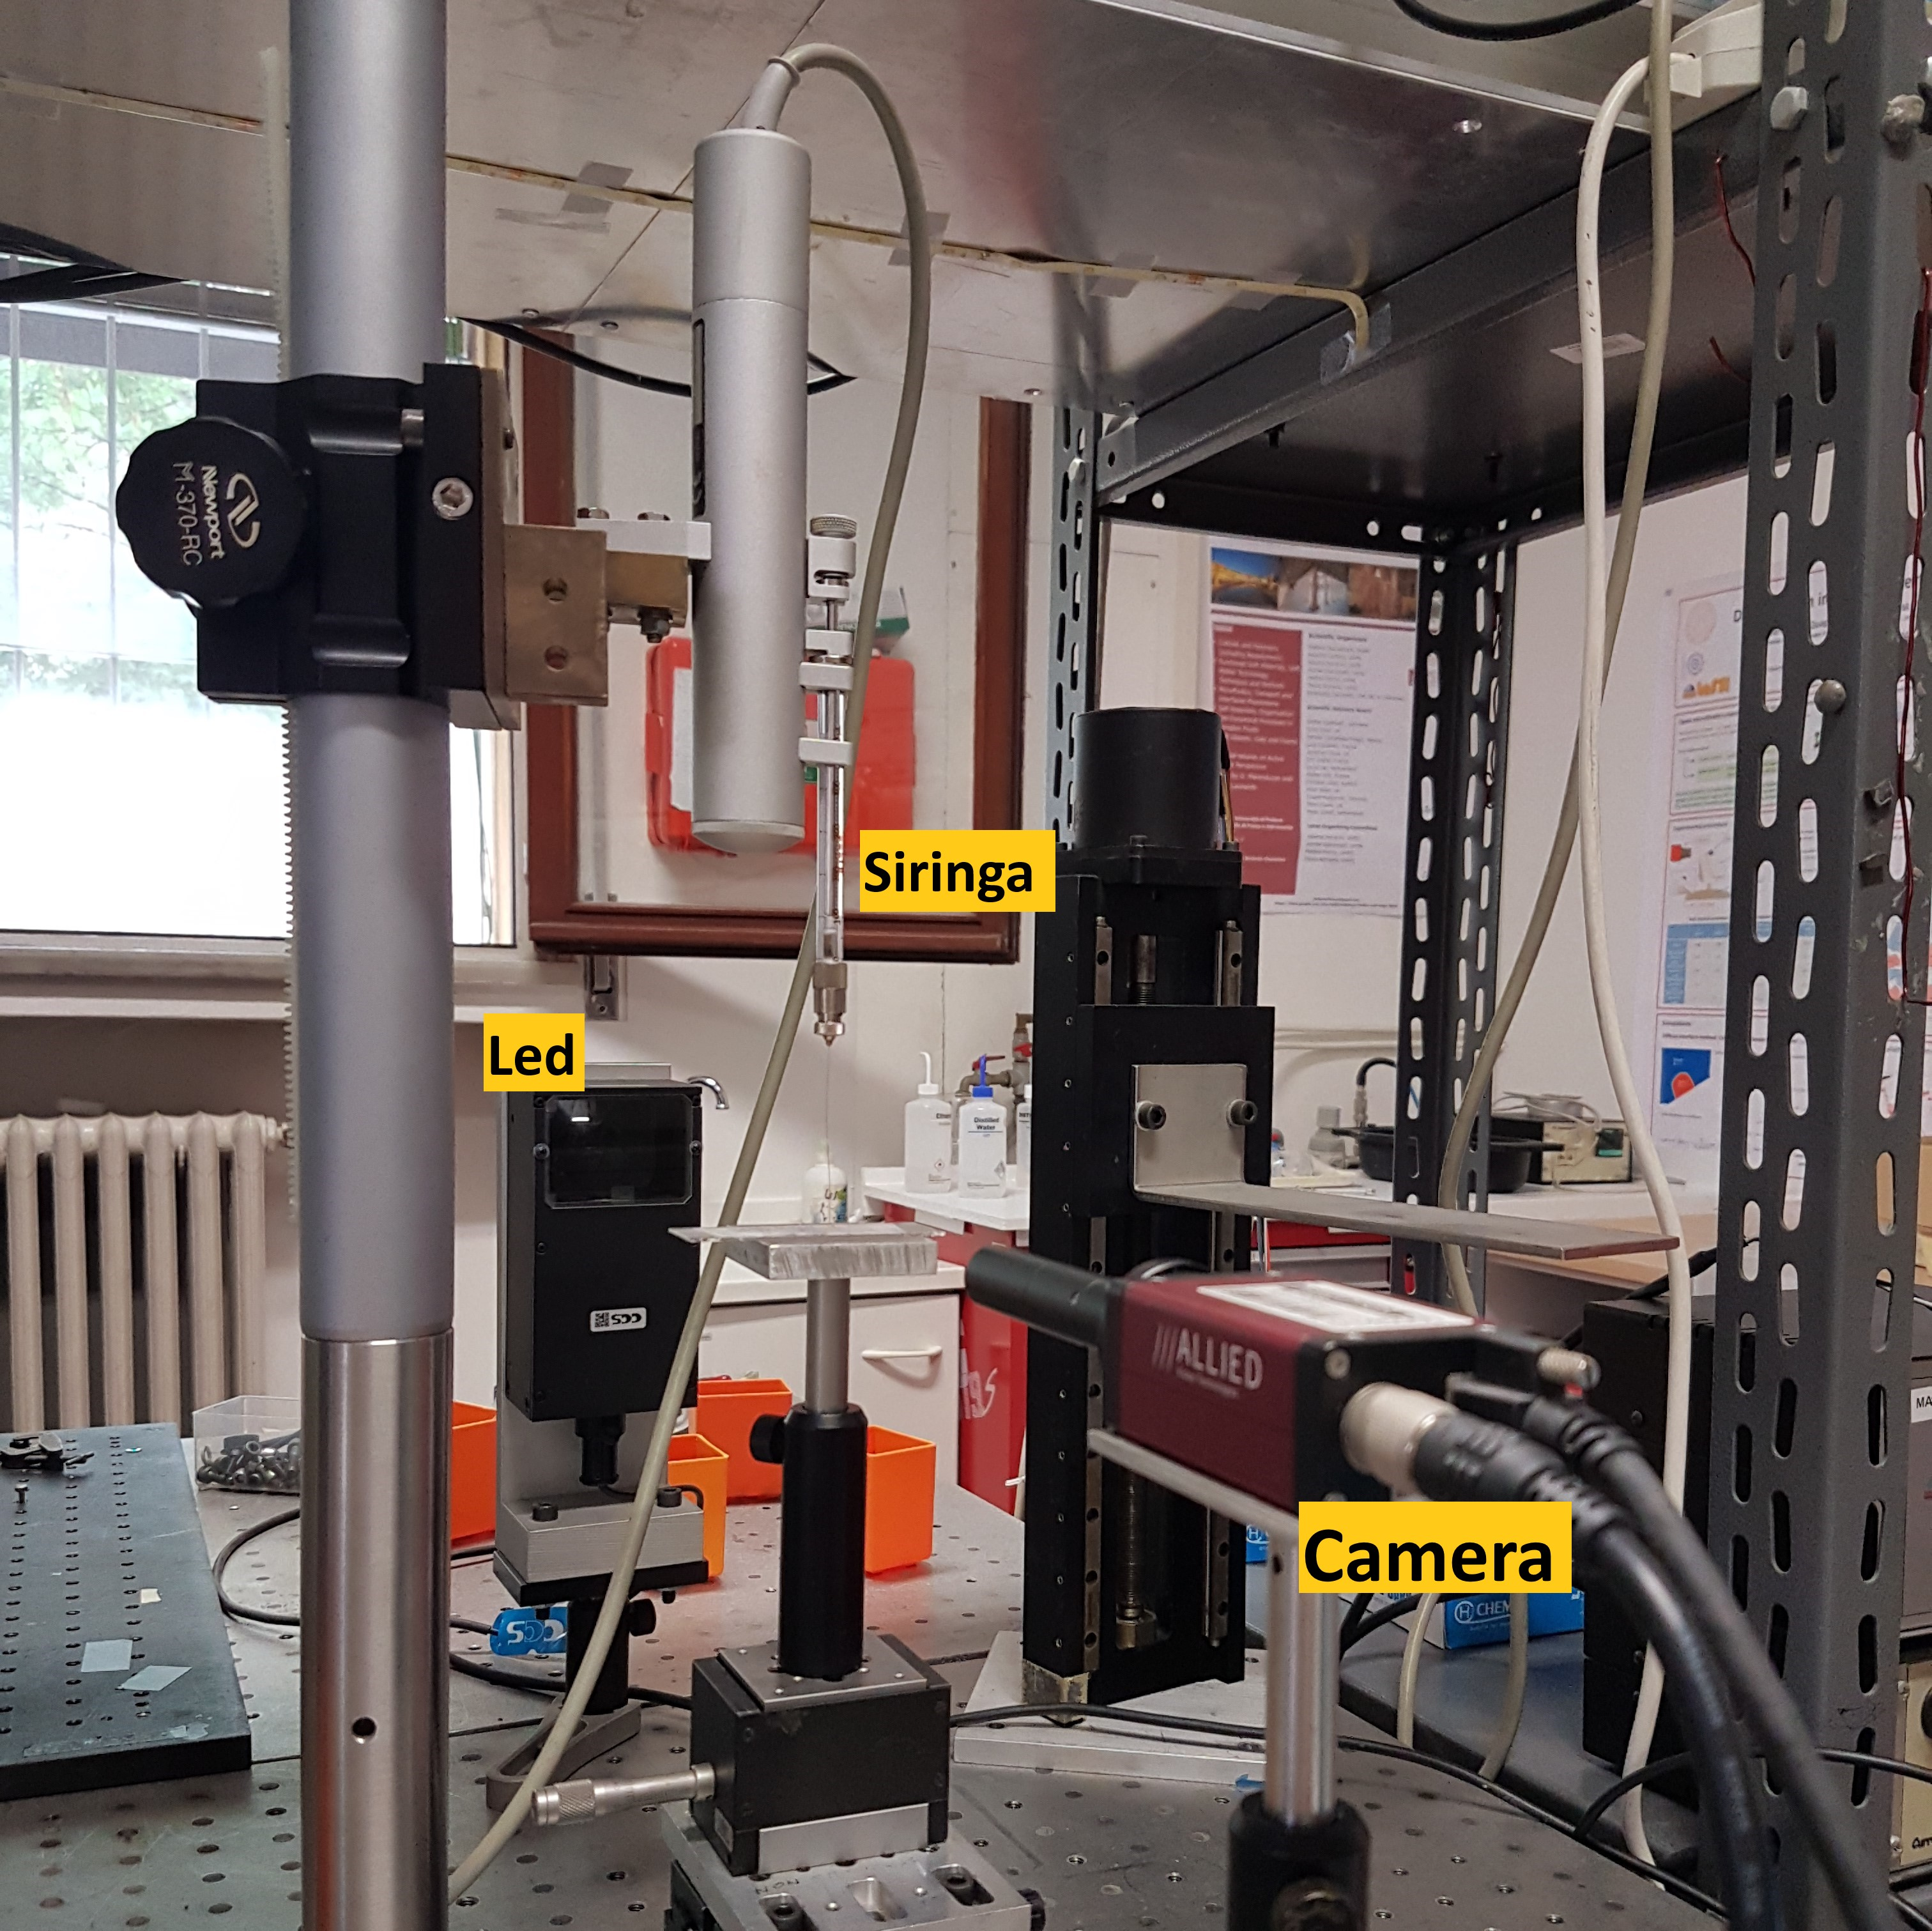
\includegraphics[width=1.0\columnwidth]{20200708_152610.jpg}
	\end{column}
	\begin{column}{.4\textwidth}
		Equipment:
		\begin{itemize}
			\item focused Led 
			\item Teflon/Parafilm
			\item  ALLIED cam + telecentric lens (425 pixel/mm)
			\item Syringe driver ($\mu L / nL$)
			\item LabView program to acquire video and angles computation	\end{itemize}
		Purposes:
		\begin{itemize}
			\item Characterization of Young angle
			\item Hysteresis measurements of contact angle to choose the substrate
			\item Standard study of surface tension with "Pendant Drop" method
		\end{itemize}
		
	\end{column}
\end{columns}

\end{frame}
%%%%%%%%%%%%%%%%%%%%%%%%%%%%%%%%%%%%%%%%%%%%%%%%%%%%%%%%%%%%%%%%%%%

\begin{frame}

\frametitle{LabView analysis}
\fontsize{8.5}{10.2} \selectfont

\begin{columns}
\begin{column}{.4\textwidth}
	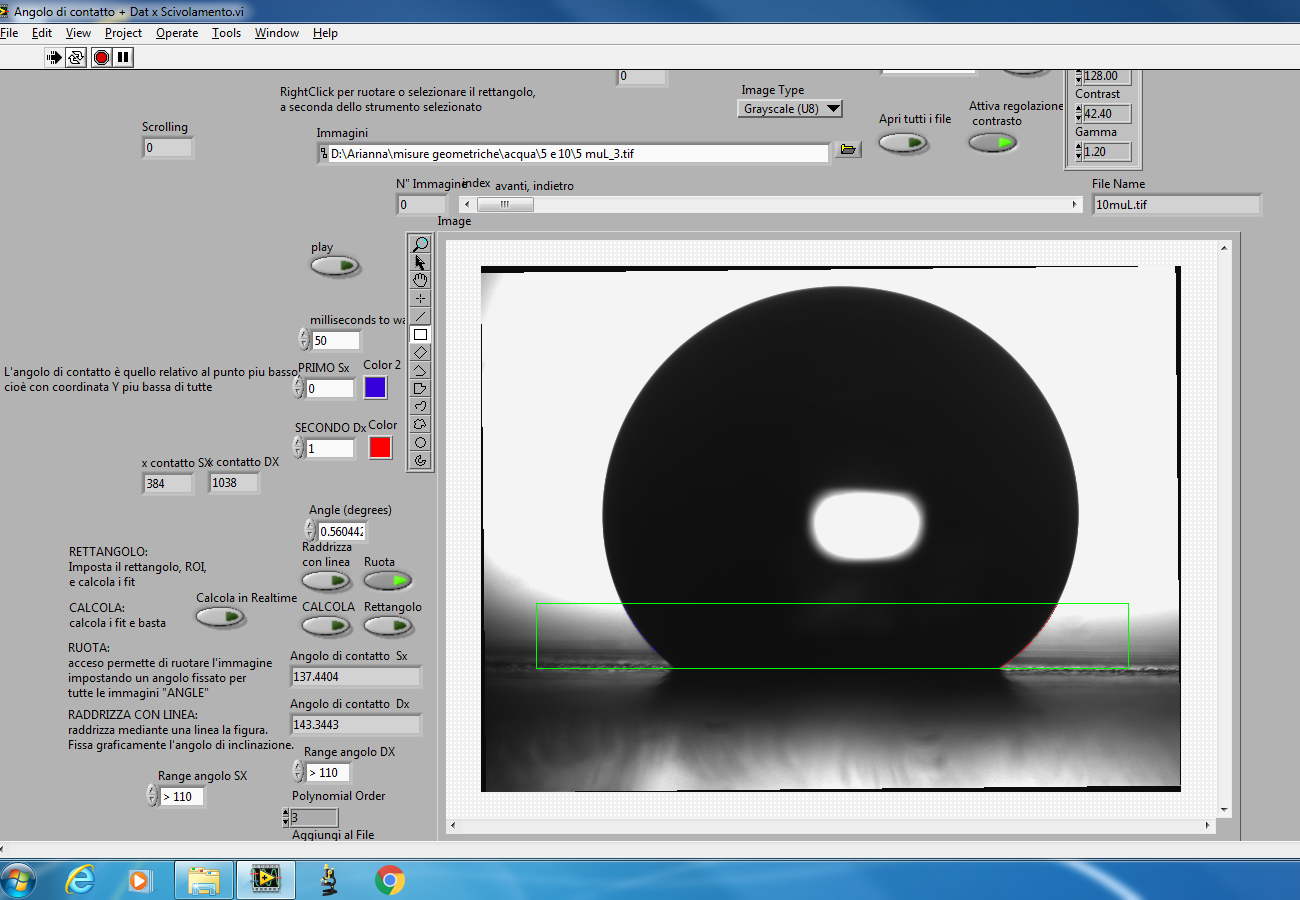
\includegraphics[width=0.95\columnwidth]{analangolo.png}\\
	\medskip
	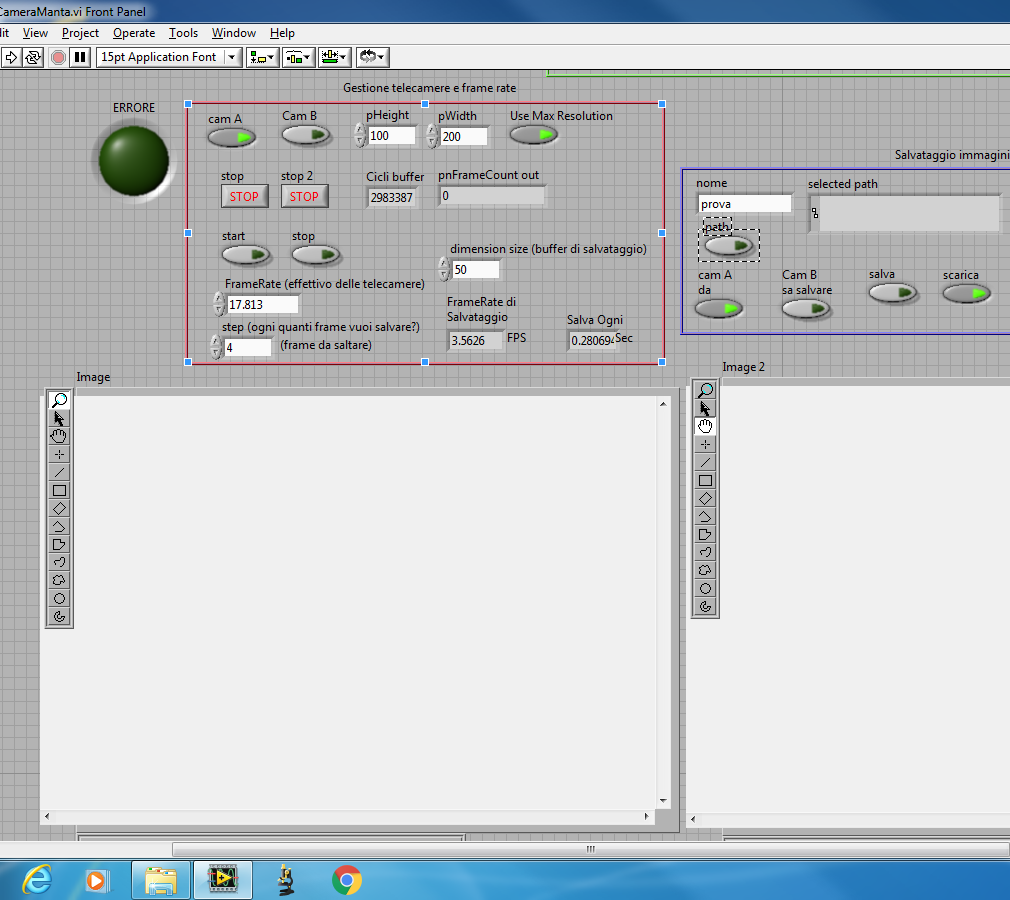
\includegraphics[width=0.95\columnwidth]{analisteresi.png}
\end{column}
\begin{column}{.5\textwidth}
	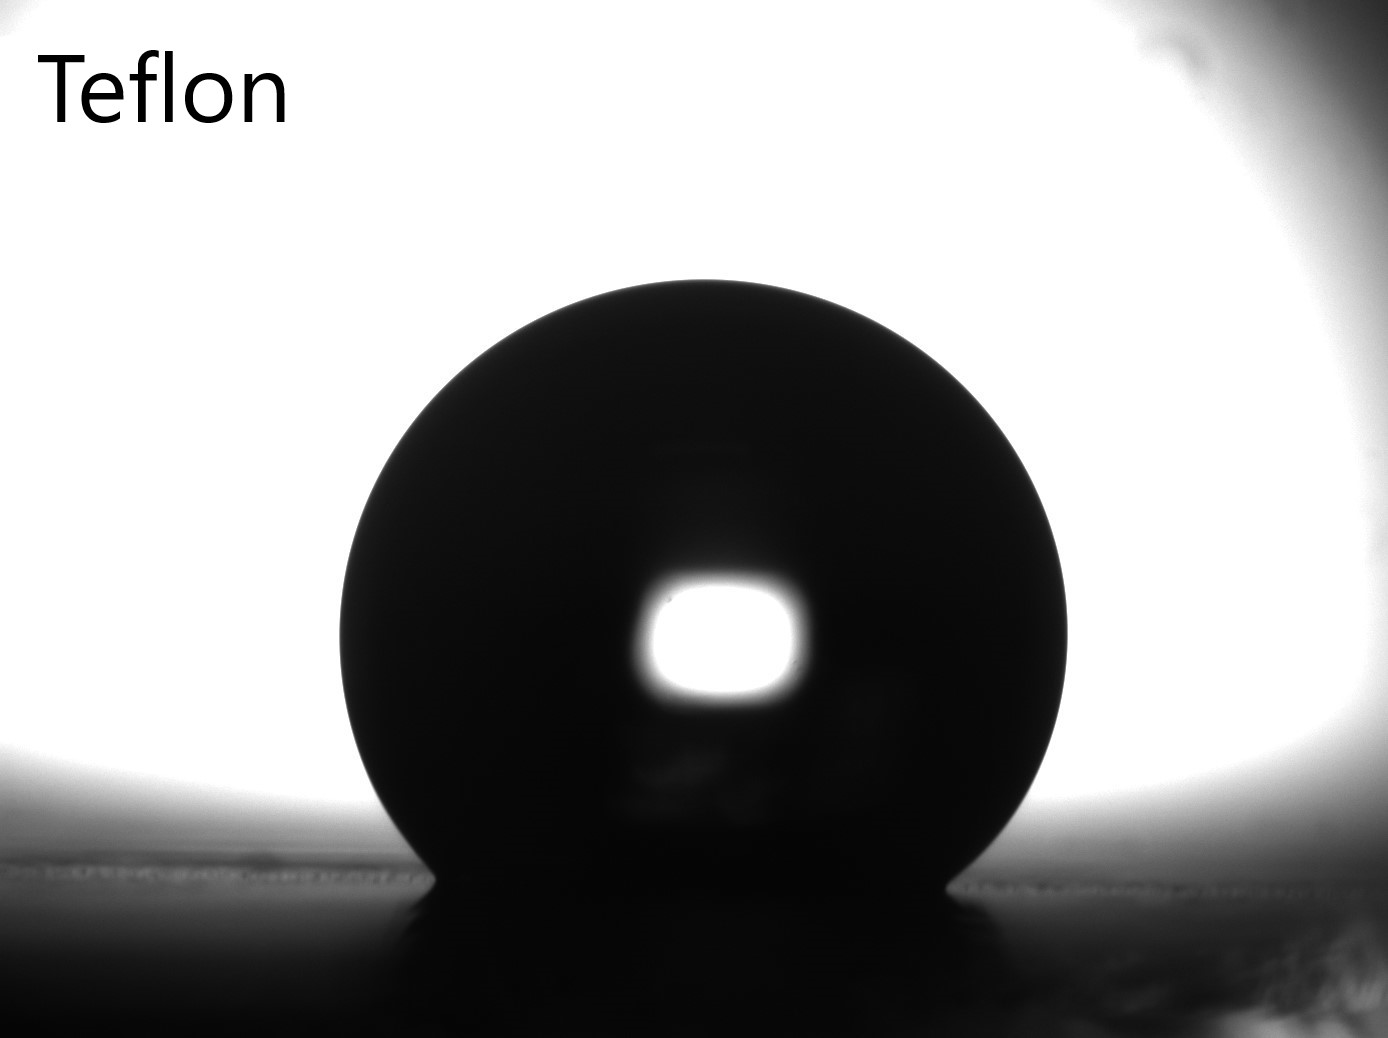
\includegraphics[width=0.5\columnwidth]{teflon_acqua_1.jpg}
	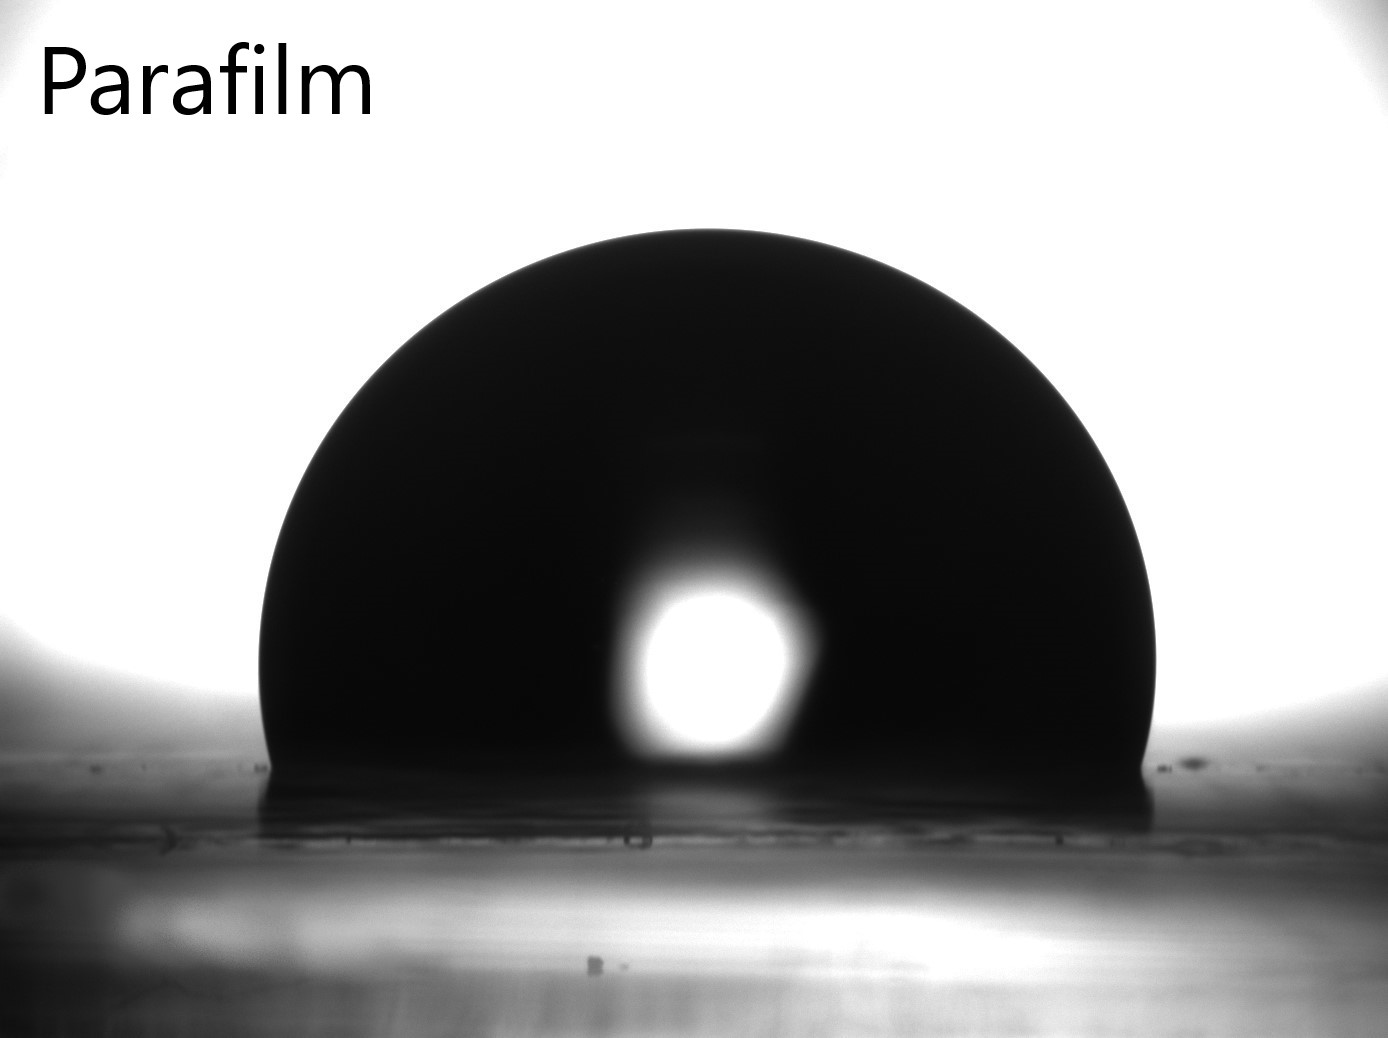
\includegraphics[width=0.5\columnwidth]{parafilm_acqua_1.jpg}\\
	UP water:
	\begin{table}[]
		\begin{tabular}{|c|c|c|c|}
			\hline
			& $\theta_{contact} $& $\theta_{reciding}$ & $\theta_{advancing}$ \\
			\hline
			Teflon   & $125^\circ \pm 4^\circ $                        & $ 59^\circ \pm 6^\circ$                         & $144^\circ \pm 3^\circ$                          \\
			Parafilm & $100^\circ \pm 4^\circ$                         & $33^\circ \pm 3^\circ$                          & $105^\circ \pm 3^\circ $      \\   
			\hline               
		\end{tabular}
	\end{table}
	Glycerol + water:
	\begin{table}[]
		\begin{tabular}{|c|c|}
			\hline
			Teflon   & $\theta_{contact}$ \\
			\hline
			gly 60\% & $127^\circ \pm 7^\circ$             \\
			gly 75\% & $133^\circ \pm 11^\circ$            \\
			gly 85\% & $134^\circ \pm 13^\circ$           \\
			\hline
		\end{tabular}
	\end{table}
\end{column}
\end{columns}

\end{frame}
%%%%%%%%%%%%%%%%%%%%%%%%%%%%%%%%%%%%%%%%%%%%%%%%%%%%%%%%%%%%%%%%%%%

\begin{frame}

\frametitle{Captured images for the hysteresis study}
\fontsize{10}{10.2} \selectfont
\centering
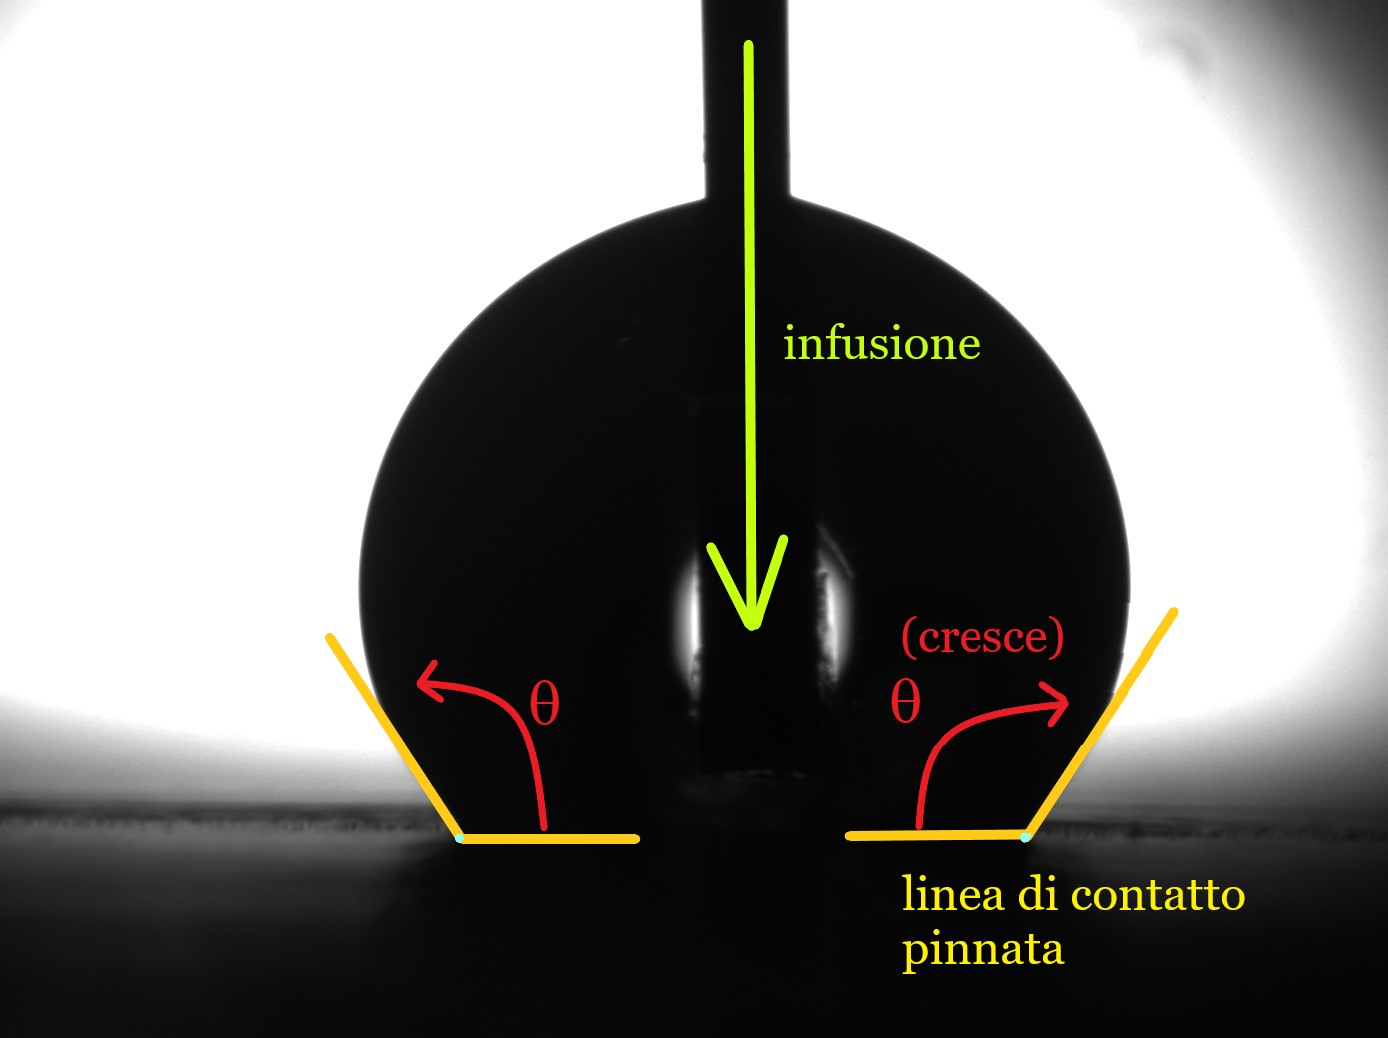
\includegraphics[width=.45\columnwidth]{isteresi1.jpg}
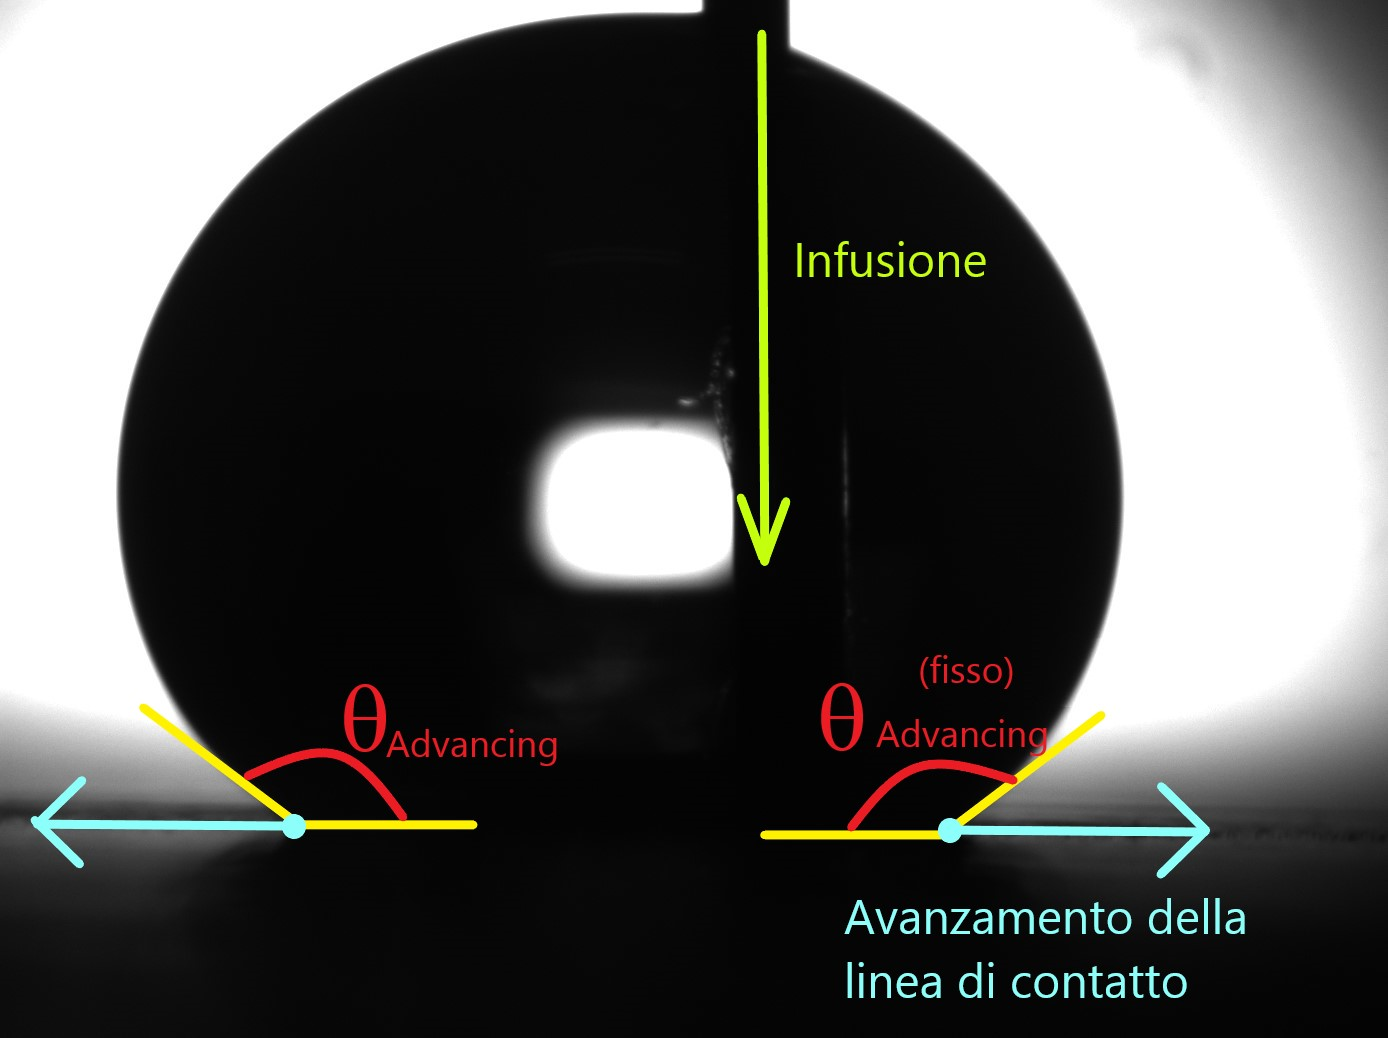
\includegraphics[width=.45\columnwidth]{isteresi2.jpg}\\
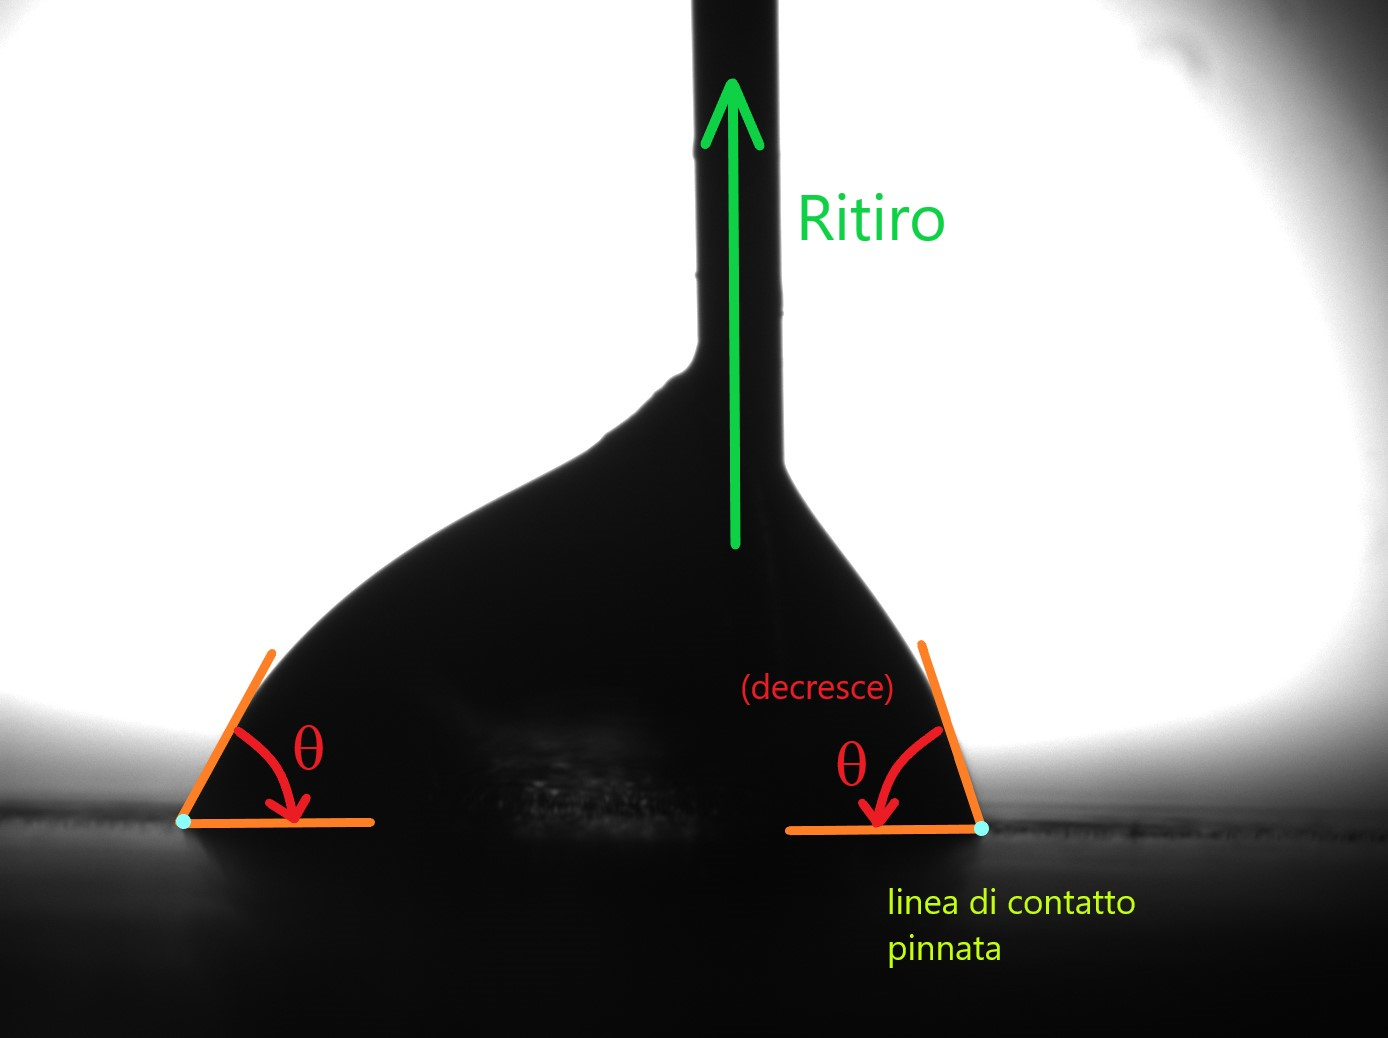
\includegraphics[width=.45\columnwidth]{isteresi3.jpg}
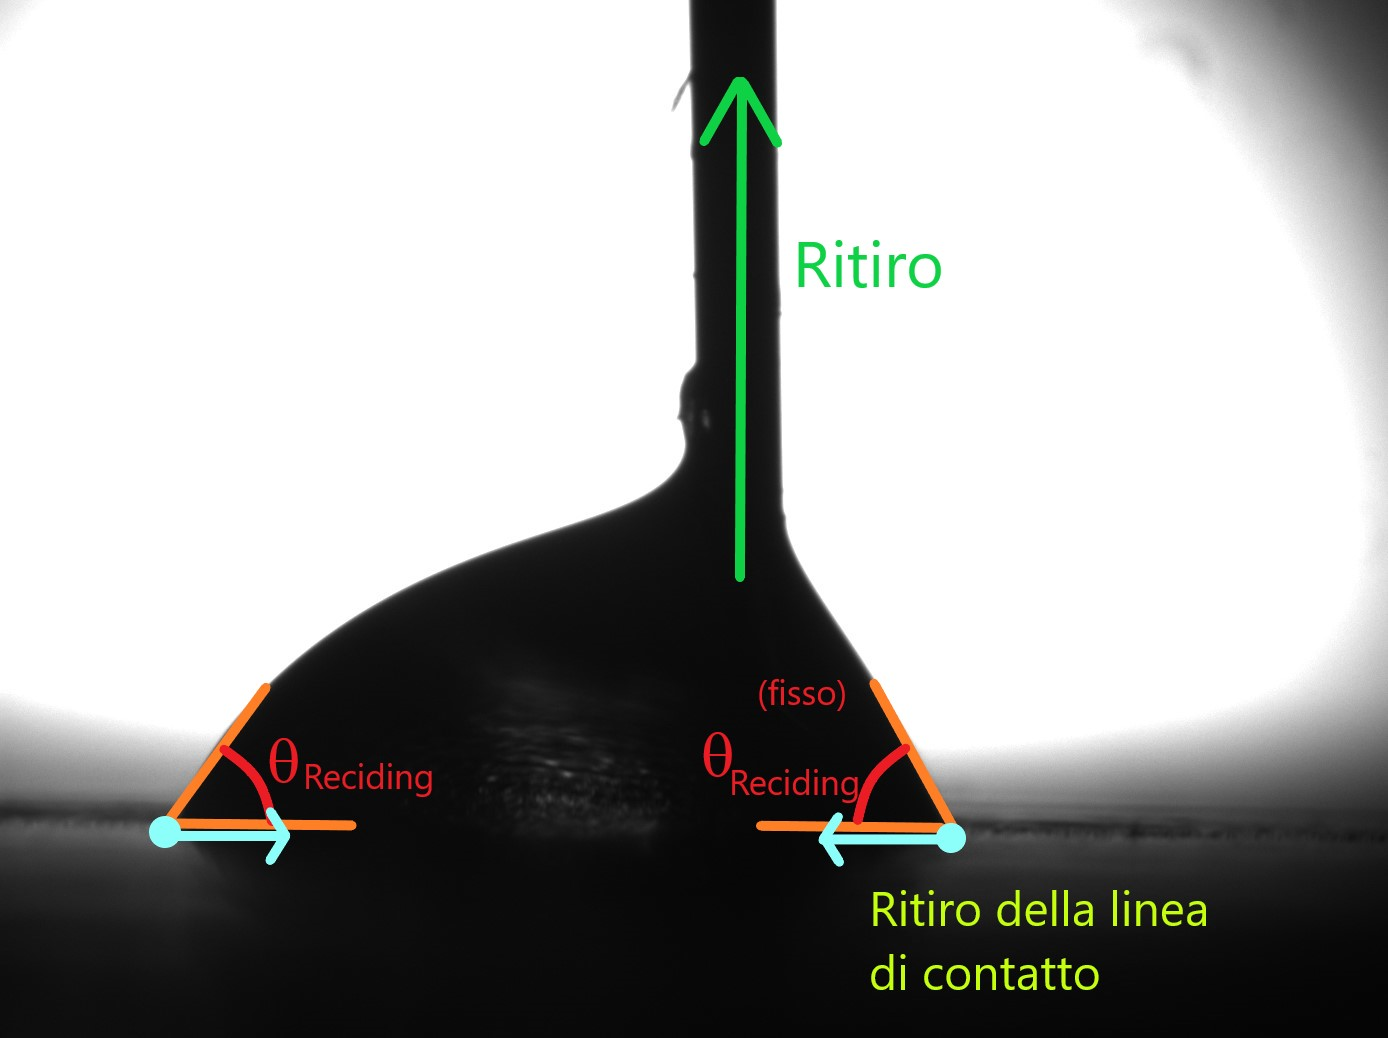
\includegraphics[width=.45\columnwidth]{isteresi4.jpg}\\

\end{frame}
%%%%%%%%%%%%%%%%%%%%%%%%%%%%%%%%%%%%%%%%%%%%%%%%%%%%%%%%%%%%%%%%%%

\begin{frame}

\frametitle{Imeagej analysis:surface tension preliminar study and droplet radius}
\fontsize{10}{10.2} \selectfont

\begin{columns}
\begin{column}{.5\textwidth}
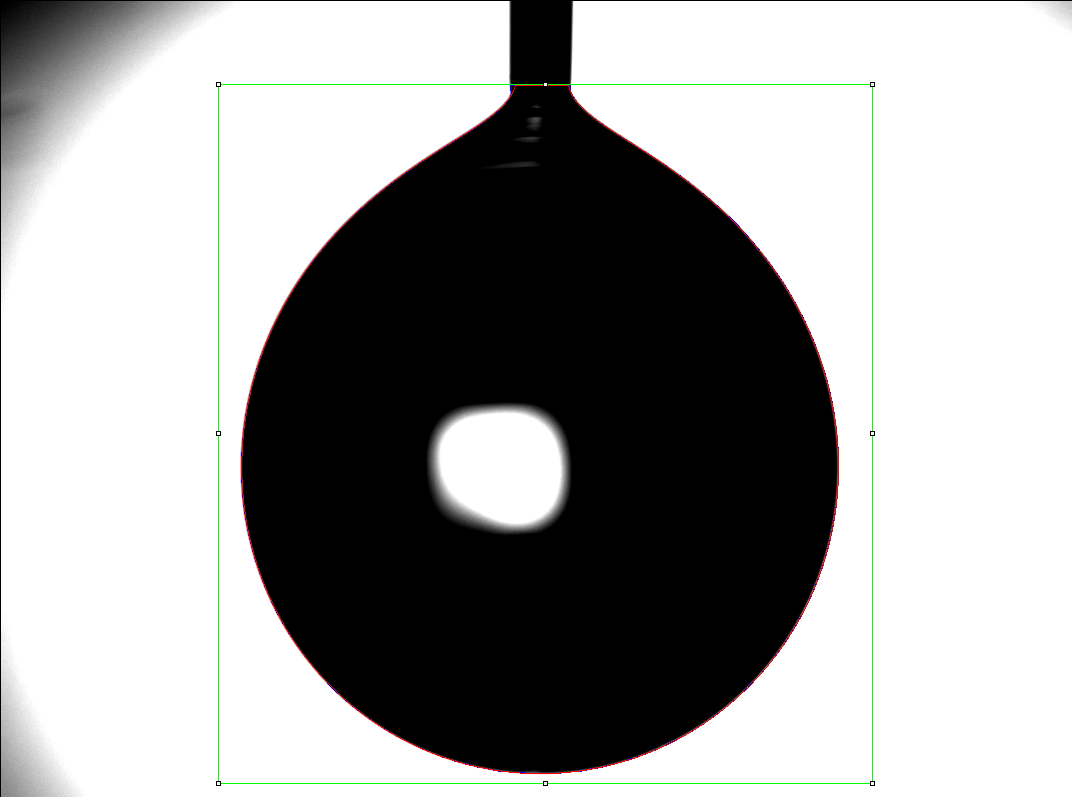
\includegraphics[width=0.95\columnwidth]{analpendandt.PNG}\\
$\uparrow$Pendent Drop profile generation and fitting\\
\medskip
Geometry of drop profile $\rightarrow$
\end{column}
\begin{column}{.5\textwidth}
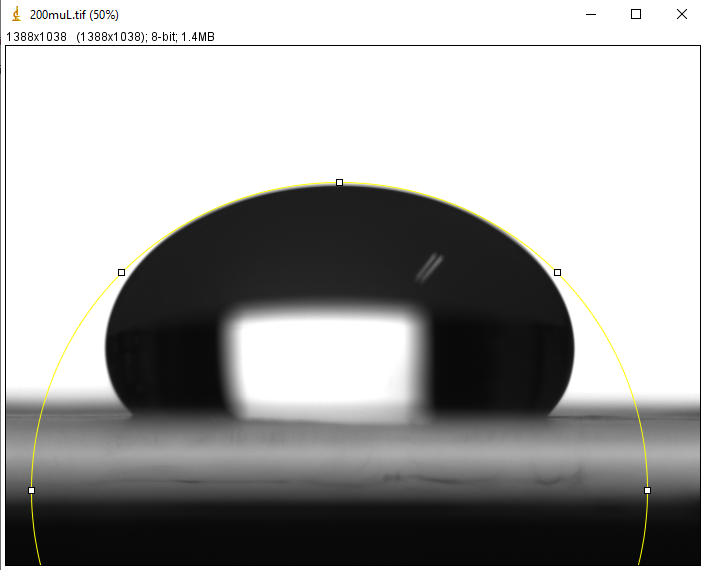
\includegraphics[width=0.8\columnwidth]{200muL.PNG}\\
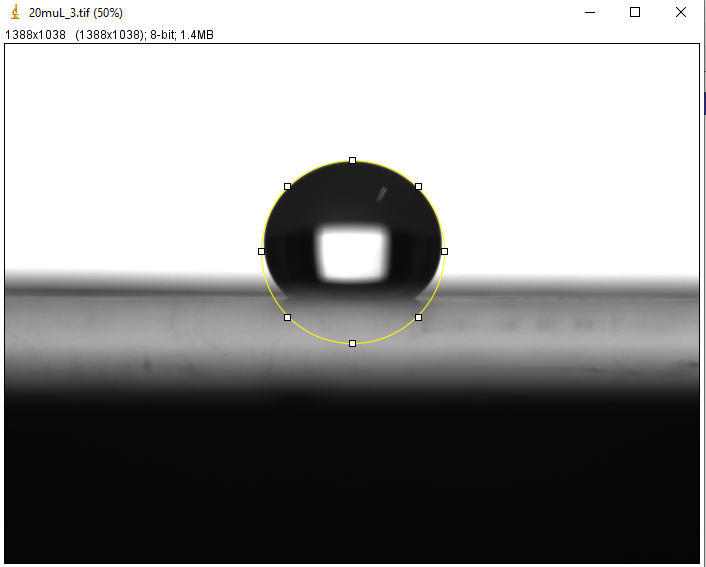
\includegraphics[width=0.8\columnwidth]{20muL.PNG}\\

\end{column}
\end{columns}
\end{frame}

%%%%%%%%%%%%%%%%%%%%%%%%%%%%%%%%%%%%%%%%%%%%%%%%%%%%%%%%%%%%%%%
%%%%%%%%%%%%%%%%%%%%%%%%%%%%%%%%%%%%%%%%%%%%%%%%%%%%%%%%%%%%%%%%%%%%%

\begin{frame}

\frametitle{Setup 2}
\fontsize{8}{10.2} \selectfont
\includegraphics[width=.8\columnwidth]{setup1.png}


\begin{columns}
	\begin{column}{.45\textwidth}
		\begin{itemize}
			\item Laser (IIIB)
			\item LED
			\item ALLIED cam with NAVITAR lens
			\item photodiode
			\item Oscilloscope
			\item Amplification circuit
			\item Data acquisition module (NATIONAL INSTRUMENT MyRio)
			\item Labview programme
		\end{itemize}
		
		
	\end{column}
	\begin{column}{.6\textwidth}
		\centering
	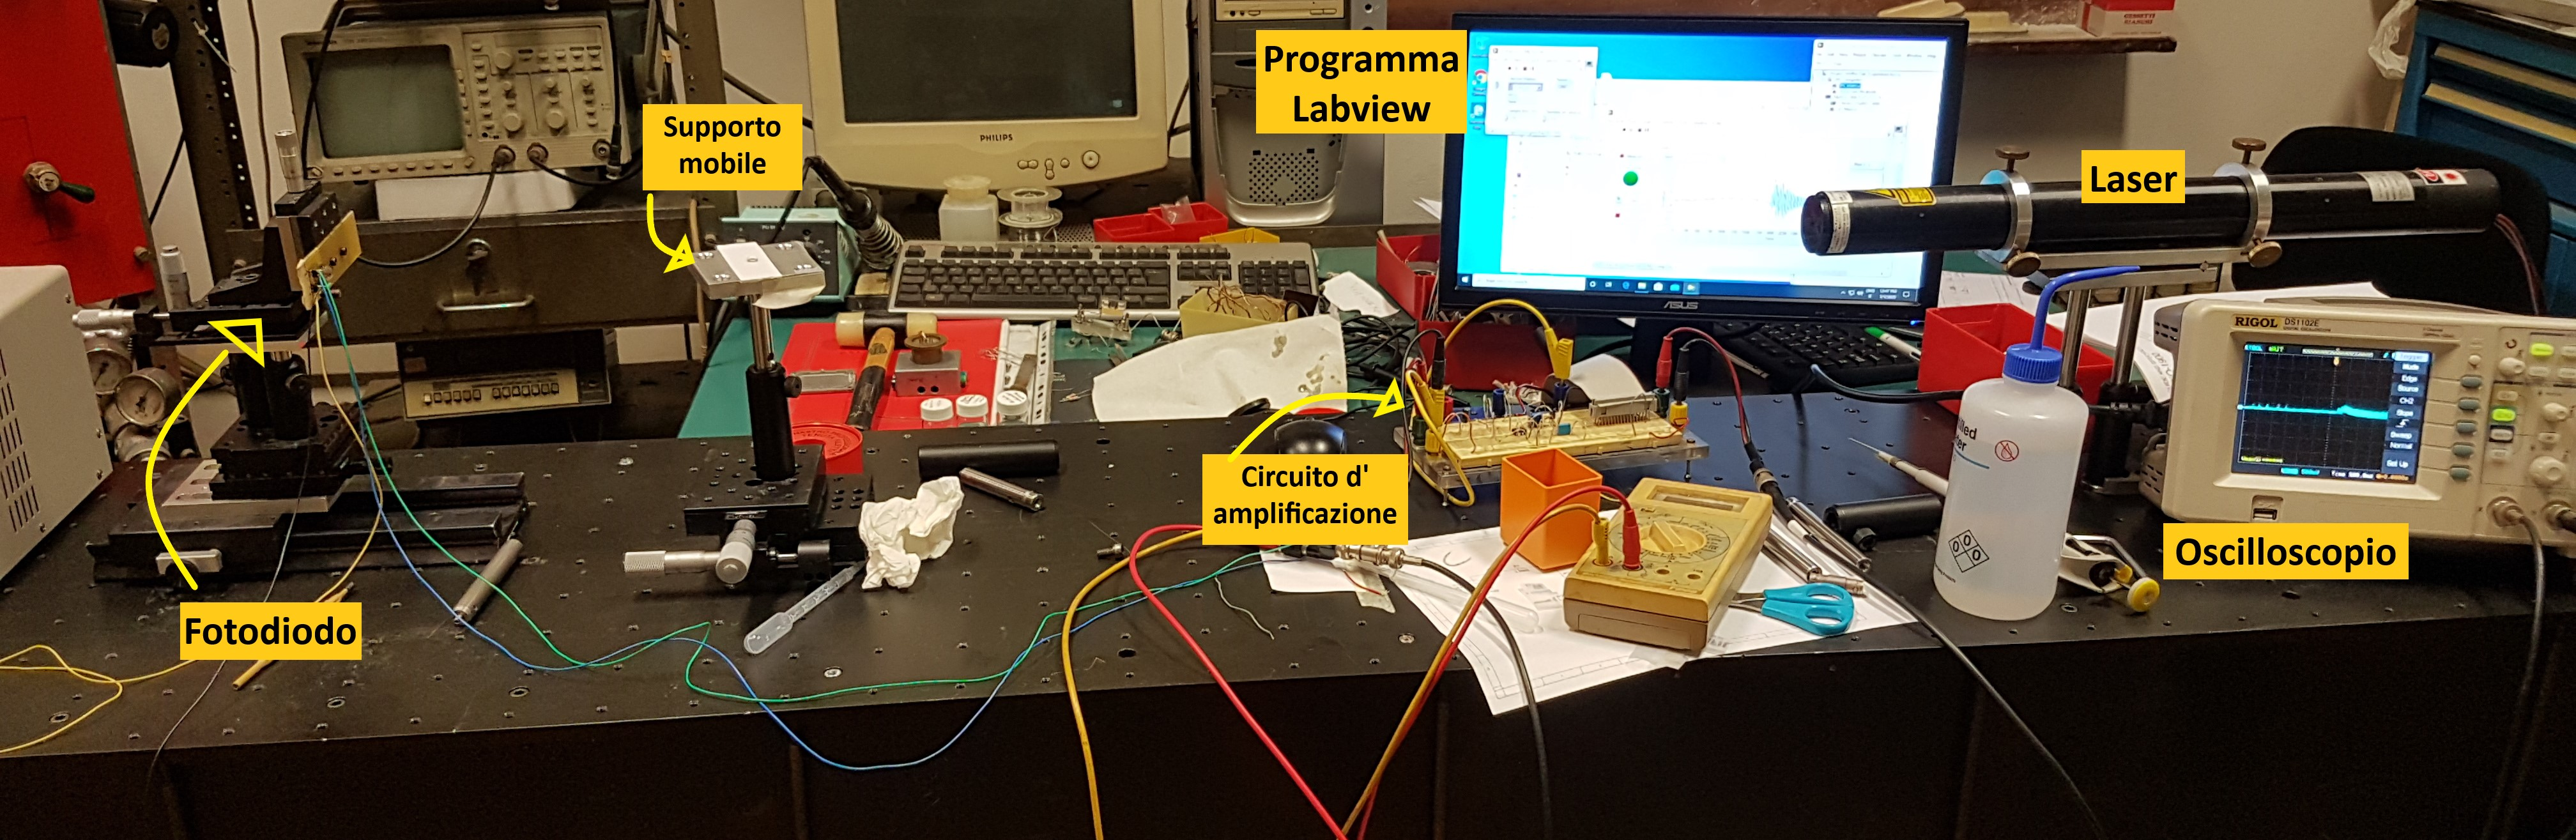
\includegraphics[width=.7\columnwidth]{20200707_124708.jpg}\\
	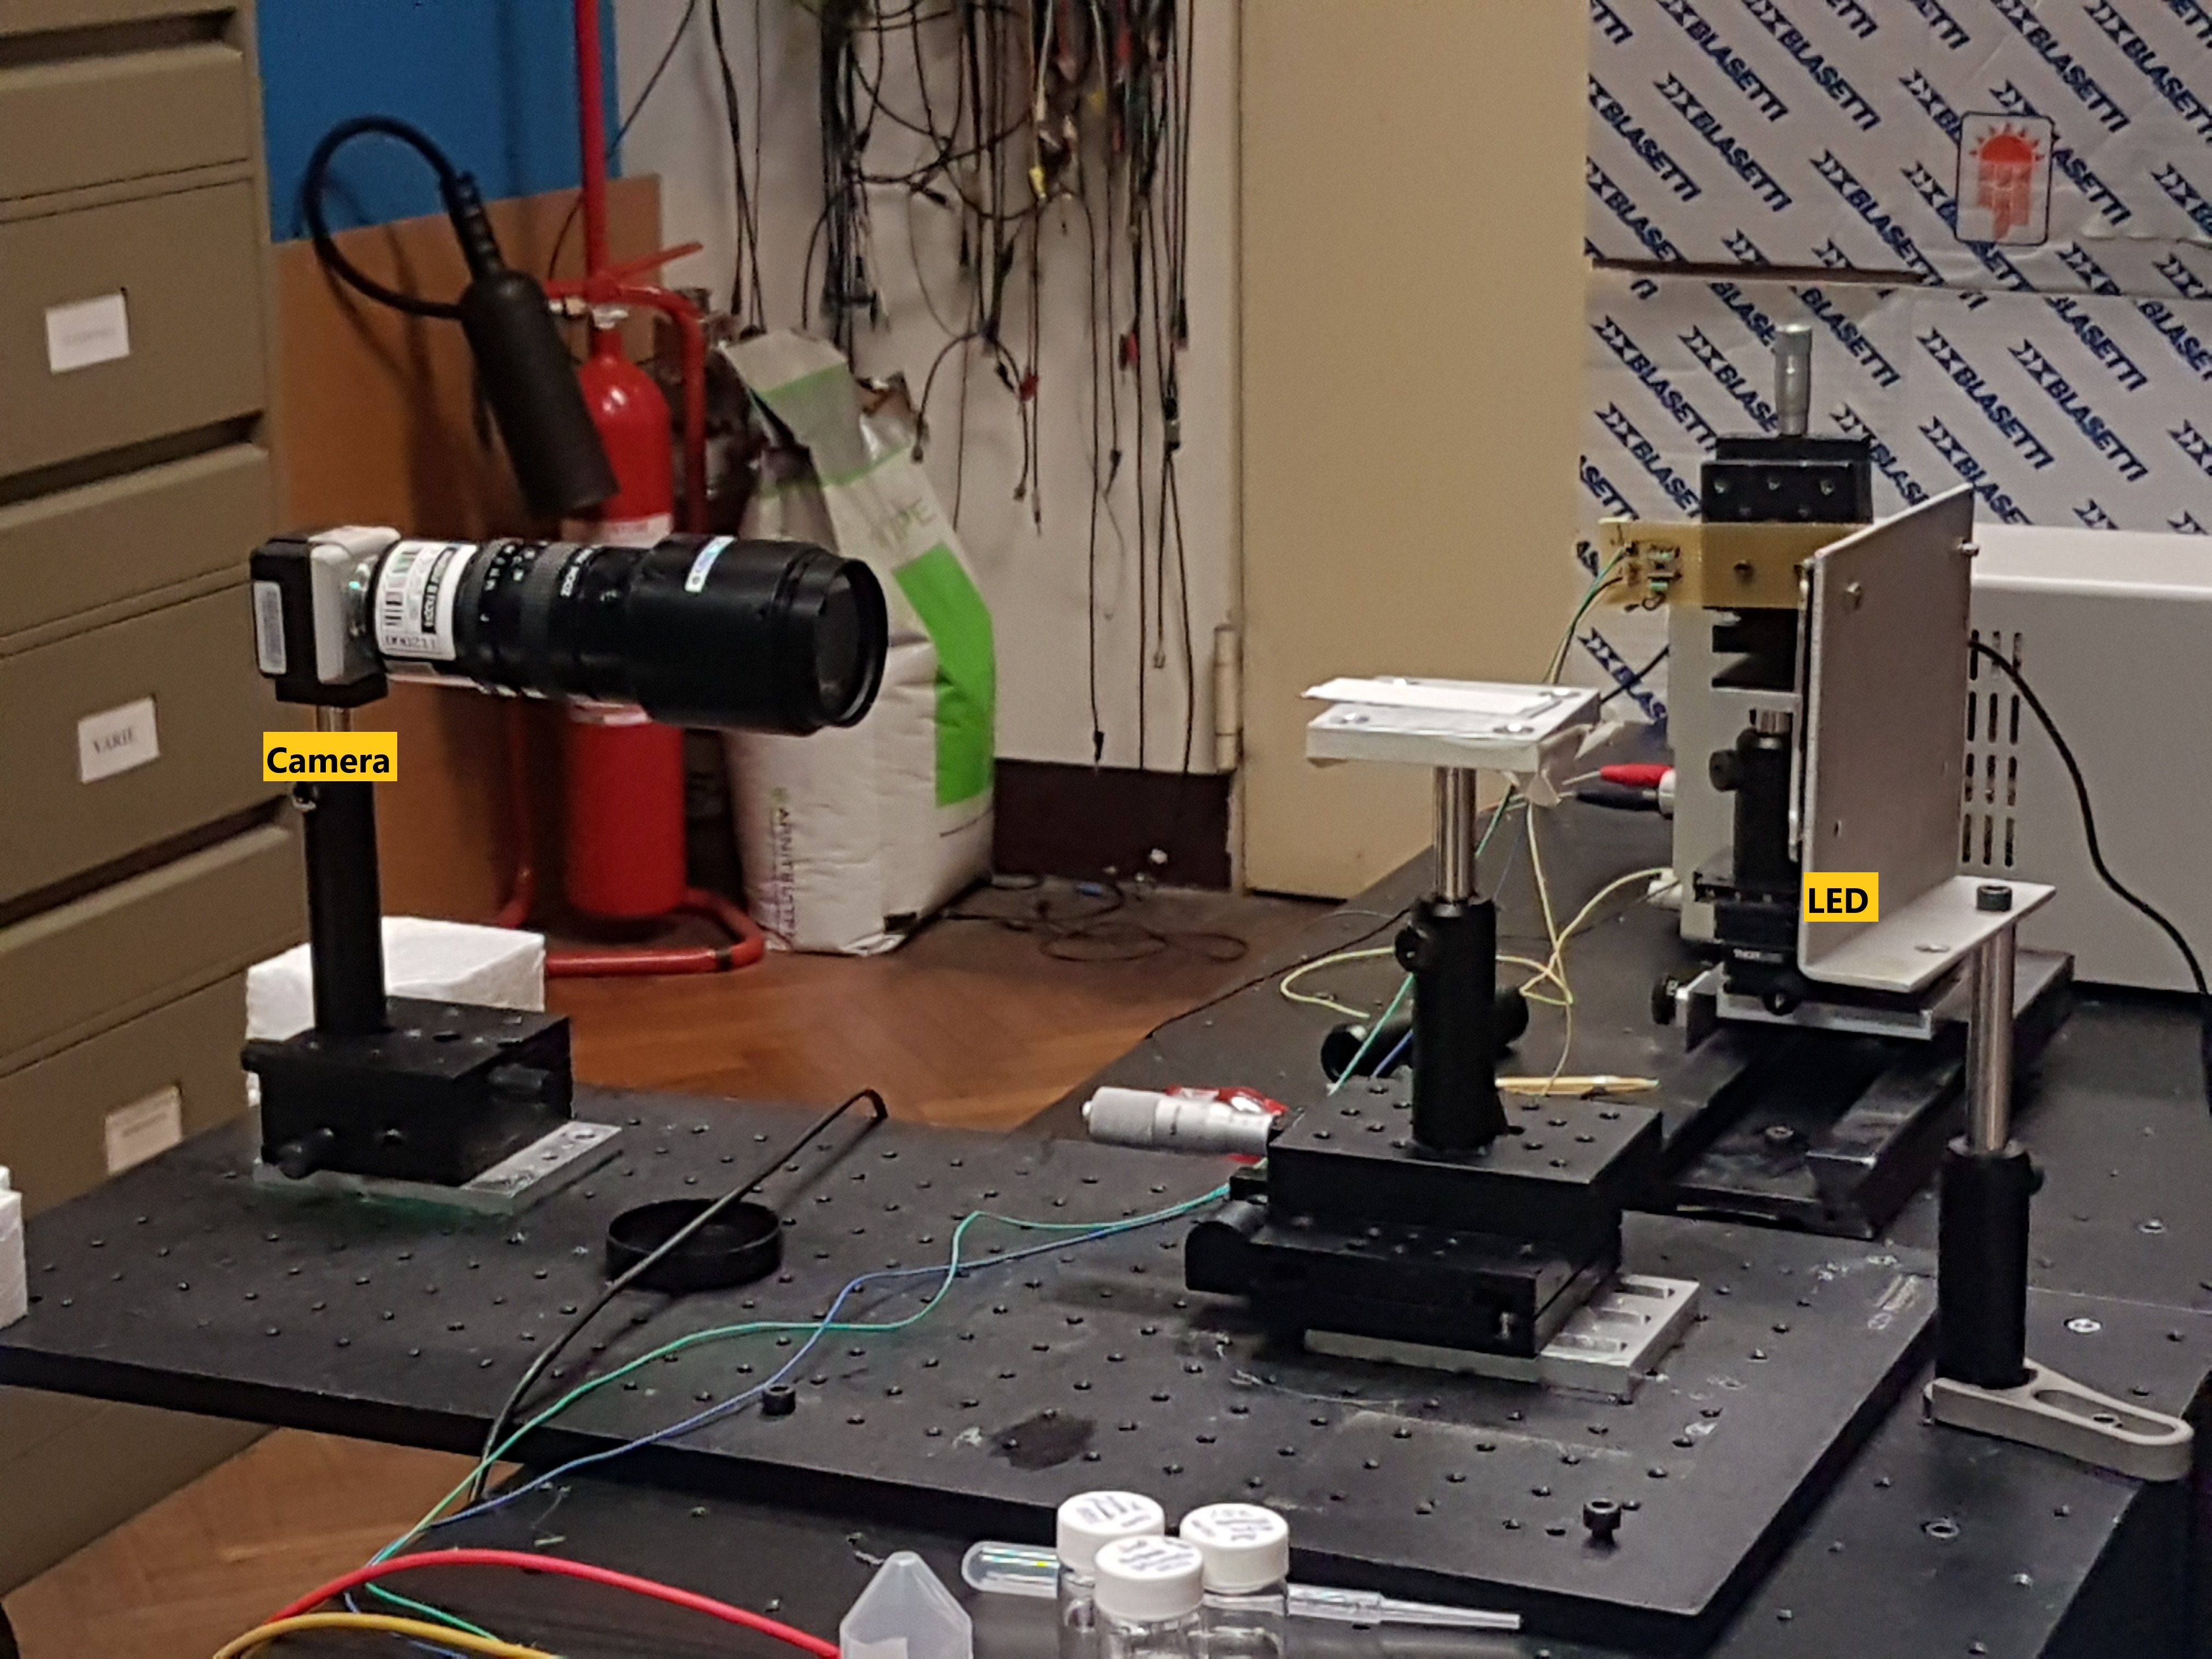
\includegraphics[width=.6\columnwidth]{20200722_105635.jpg}\\	
	\end{column}
\end{columns}

\end{frame}

%%%%%%%%%%%%%%%%%%%%%%%%%%%%%%%%%%%%%%%%%%%%%%%%%%%%%%%%%
\begin{frame}
\frametitle{Setup 2}
	\fontsize{8}{10.2} \selectfont
	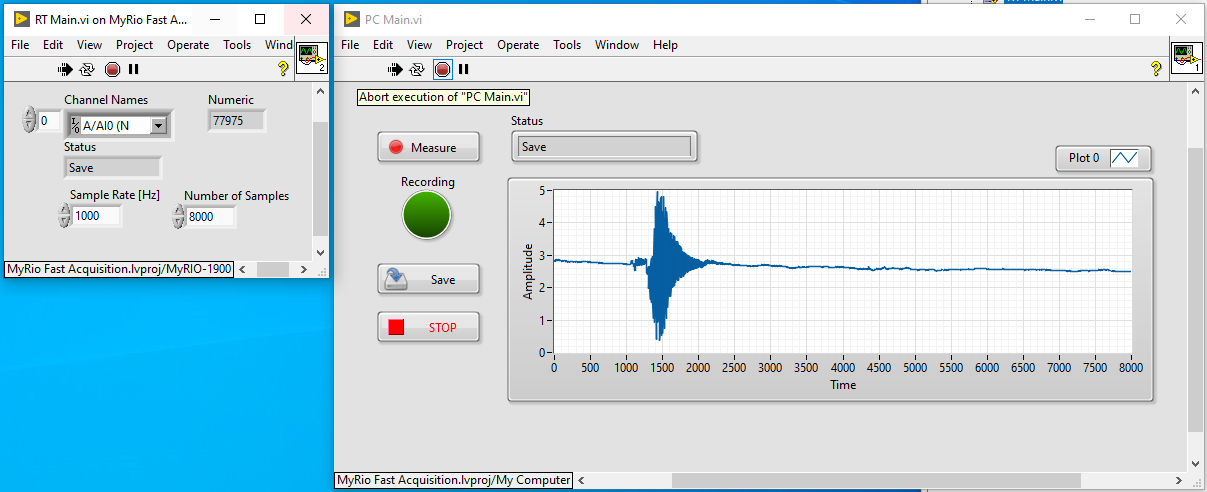
\includegraphics[width=.8\columnwidth]{Labview_programme.PNG}\\
	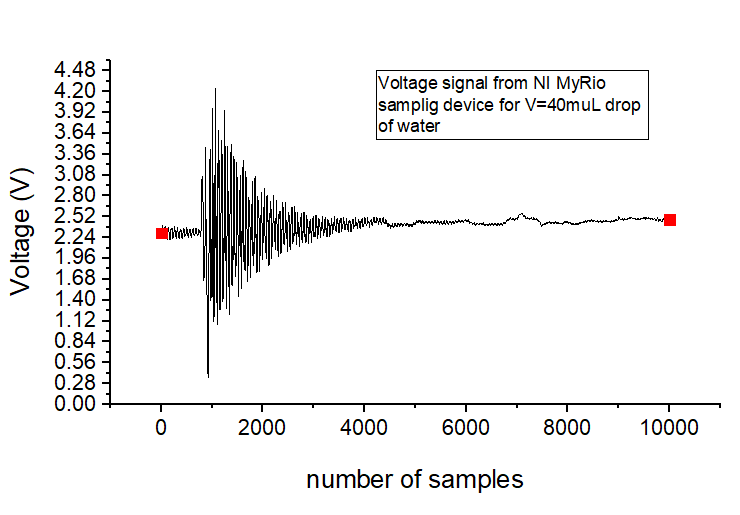
\includegraphics[width=.5\columnwidth]{voltagesignal.PNG}
	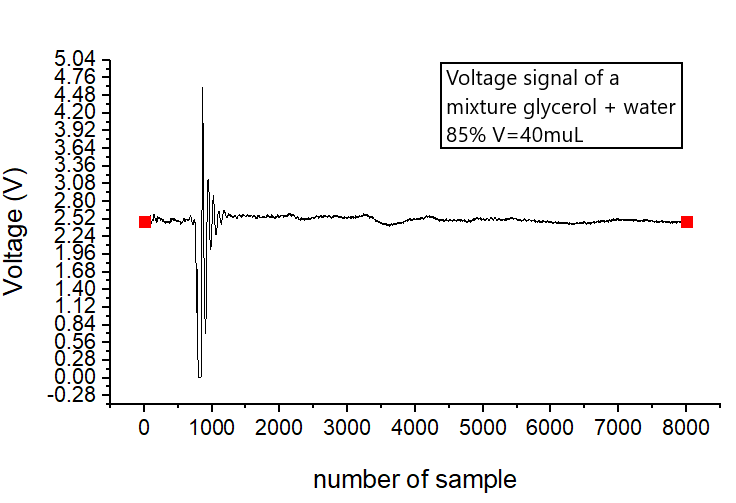
\includegraphics[width=.5\columnwidth]{voltaggio8540muL.PNG}\\ 
\end{frame}

%%%%%%%%%%%%%%%%%%%%%%%%%%%%%%%%%%%%%%%%%%%%%%%%%%%%%%%%%%%%%%%%%%%%%%%
\begin{frame}

\frametitle{UP water results}
\fontsize{10}{10.2} \selectfont
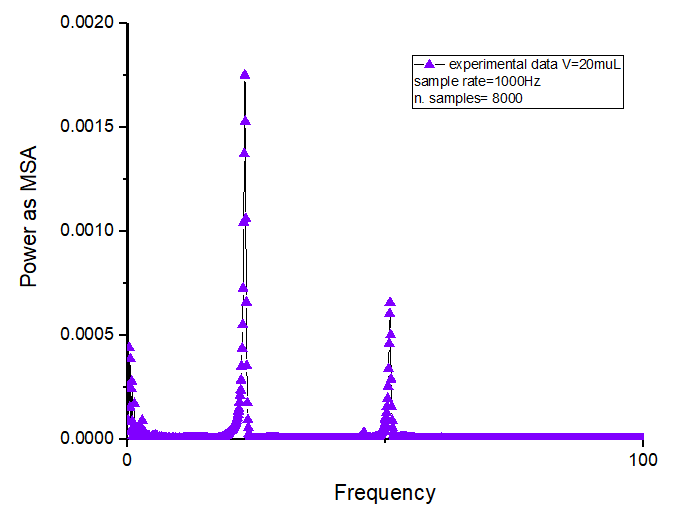
\includegraphics[width=.45\columnwidth]{20mull.png}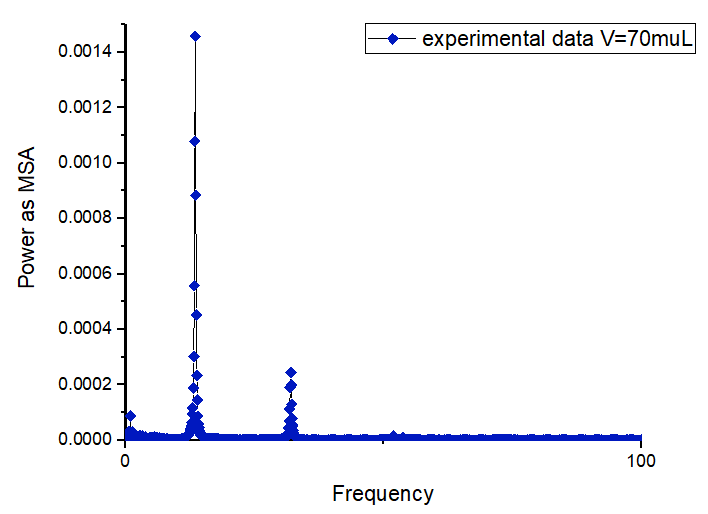
\includegraphics[width=.45\columnwidth]{70mull.png}\\
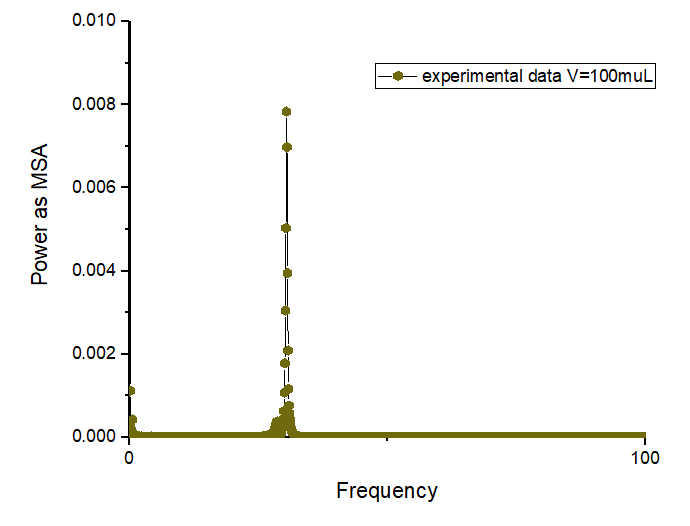
\includegraphics[width=.45\columnwidth]{100mull.png}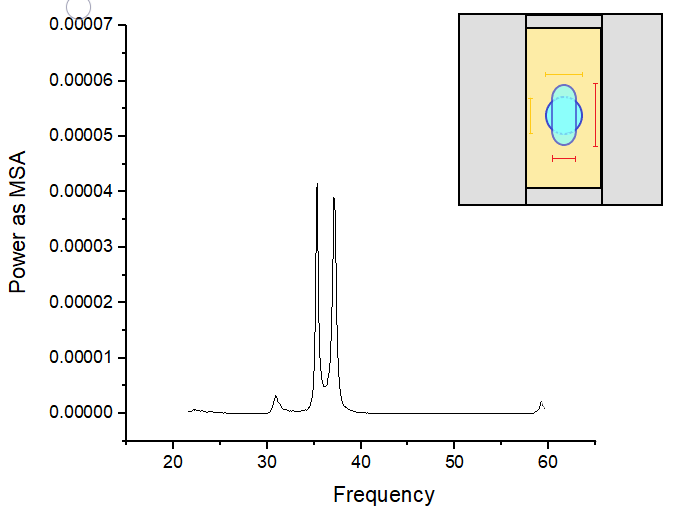
\includegraphics[width=.45\columnwidth]{picco_sdoppiato.png}
\end{frame}

%%%%%%%%%%%%%%%%%%%%%%%%%%%%%%%%%%%%%%%%%%%%%%%%%%%%%%%%%%%%%%%%%%%%%
\begin{frame}
\frametitle{Peak Analizer}

\fontsize{10}{10.2} \selectfont
Peak Analizer by Origin
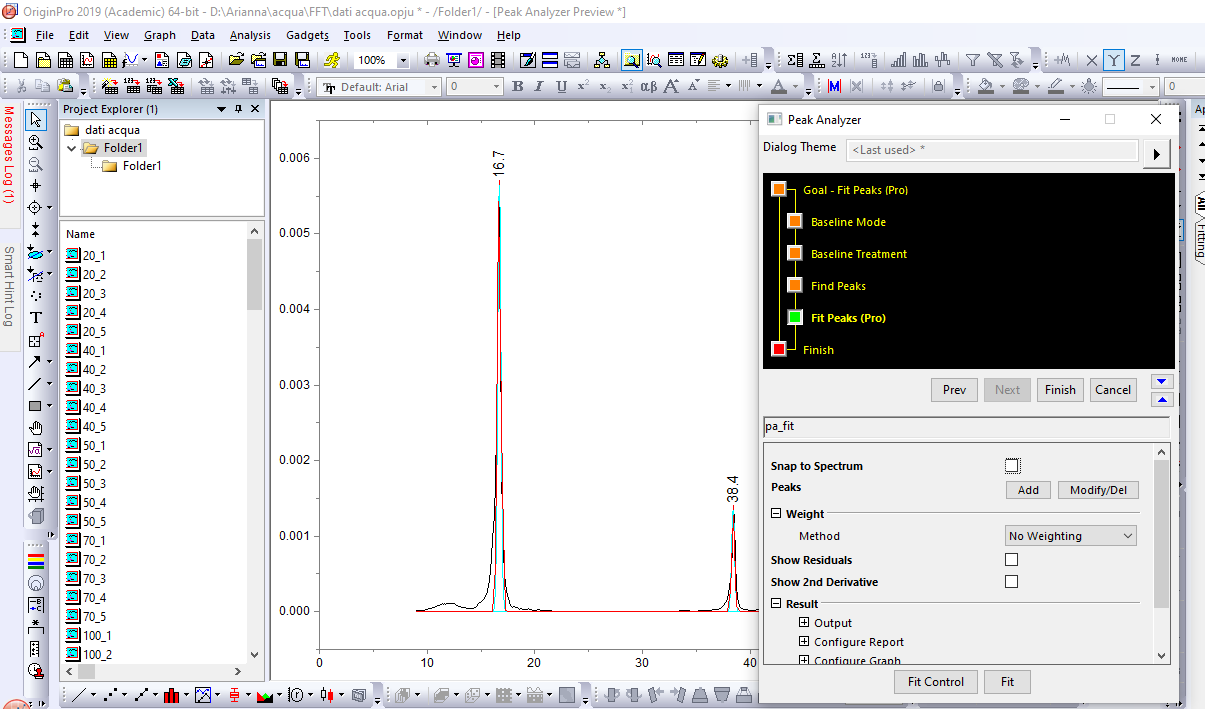
\includegraphics[width=.9\columnwidth]{peak_analizer.PNG}

\end{frame}
%%%%%%%%%%%%%%%%%%%%%%%%%%%%%%%%%%%%%%%%%%%%%%%%%%%%%%%%%%%%%%%%%%%%%%%%%%%%%%%

\begin{frame}
\frametitle{UP water results}
\fontsize{10}{10.2} \selectfont
Frequencies with Sharp's formula (Hz):
\fontsize{7}{10.2} \selectfont
	\begin{table}
			\begin{tabular}{|c|c|c|c|c|c|} 
				\hline
				\multicolumn{1}{|c|}{} &\multicolumn{1}{|c|}{$20 \mu L$} &\multicolumn{1}{|c|}{$40 \mu L$} &\multicolumn{1}{|c|}{$50 \mu L$} &\multicolumn{1}{|c|}{$70 \mu L$} & \multicolumn{1}{c|}{$100 \mu L$} \\
				\rowcolor[HTML]{FFFC9E} 
				\hline
				n=2  &   $24,5 \pm 0,02$ & $ 17,3 \pm0,01 $ & $ 15,5 \pm0,01$ & $13,09\pm0,008$ &  $	10,96 \pm 0,007$\\
				
				\hline
			\end{tabular}
	\end{table}	
\fontsize{10}{10.2} \selectfont
Frequencies with Temperton's formula (Hz):
\fontsize{7}{10.2} \selectfont
			\begin{table}[]
				\begin{tabular}{|c|c|c|c|c|c|} 
					\hline
					& 20$\mu L$  & 40$\mu L$    & 50$\mu L$   & 70$\mu L$ & 100$\mu L$   \\
					\rowcolor[HTML]{FFFC9E} 
					\hline									
					n=2 & $23,51 \pm 0,01$ & $16,624\pm0,007$ & $14,869 \pm 0,006$ & $12,567 \pm 0,004$ & $ 10,514 \pm 0,003$ \\
					\hline
				\end{tabular}
			\end{table}
		\fontsize{10}{10.2} \selectfont
Experimental resonant frequencies (Hz):
\fontsize{7}{10.2} \selectfont
\begin{table}[]
	\begin{tabular}
		{|c|c|c|c|c|c|} 
		\hline
		& 20$\mu L$  & 40$\mu L$    & 50$\mu L$   & 70$\mu L$ & 100$\mu L$   \\
		\rowcolor[HTML]{FFFC9E} 
		\hline		
		n=2 & $23,8 \pm 0,6 $  & $17,0 \pm 0,3$  & $15,3 \pm 0,4$  & $13,47 \pm 0,9$ &        \\
		\hline
	\end{tabular}
\end{table}
\end{frame}
%%%%%%%%%%%%%%%%%%%%%%%%%%%%%%%%%%%%%%%%%%%%%%%%%%%%%%%%%%%%%%%%%%%%%%


\begin{frame}

\frametitle{UP water results}
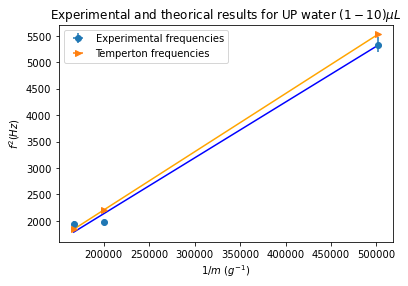
\includegraphics[width=.5\columnwidth]{Volumi_piccoli.PNG}
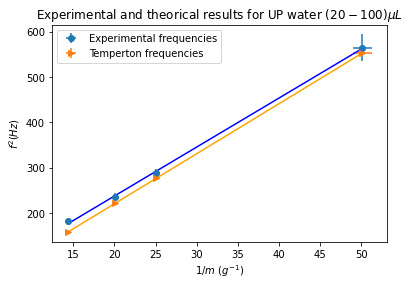
\includegraphics[width=.55\columnwidth]{volumi_grandi.PNG}\\

\end{frame}%%%%%%%%%%%%%%%%%%%%%%%%%%%%%%%%%%%%%%%%%%%%%%%%%%%%%%%%%%%%%%%%%%%%%
\begin{frame}
\frametitle{glycerol+water results}
\fontsize{7}{10.2} \selectfont
\begin{table}[]
	\begin{tabular}{|c|c|c|c|c|c|}
		\hline
		gly 60\% & 20$\mu L$  & 40$\mu L$    & 50$\mu L$   & 70$\mu L$ & 100$\mu L$   \\
		\hline
		th. (Hz) & $21,13 \pm 0,01$ & $14,941 \pm 0,008$ & $13,364 \pm 0,007$            & $11,295 \pm 0,005$ & $9,451 \pm 0,004$ \\
		exp (Hz) & $20,2 \pm 0,6$   & $14,1 \pm 0,2$     & $12,7 \pm 0,8$ &                    &                \\             
		\hline    
	\end{tabular}
\end{table}

\begin{table}[]
	\begin{tabular}{|c|c|c|c|c|c|}
		\hline
		gly 75\% & 20$\mu L$  & 40$\mu L$    & 50$\mu L$   & 70$\mu L$ & 100$\mu L$   \\
		\hline
		th. (Hz)  & $20,36 \pm 0,01$ & $ 14,396 \pm 0,009 $ & $12,876 \pm 0,008$ & $10,882 \pm 0,007$ & $9,105 \pm 0,006$ \\
		exp (Hz)                         & $19,5 \pm 0,6$   & $13,99 \pm 0,8$      &                    & $11,46 \pm 0,6$    & $ \simeq 11,1281$ \\
		\hline             
	\end{tabular}
\end{table}

\begin{table}[]
	\begin{tabular}{|c|c|c|c|c|c|}
		\hline
		gly 85\% & 20$\mu L$  & 40$\mu L$    & 50$\mu L$   & 70$\mu L$ & 100$\mu L$   \\
		\hline
		th. (Hz) & $20,06 \pm 0,01$ & $ 14,191 \pm 0,009 $ & $12,683 \pm 0,008$ & $10,728 \pm 0,007$ & $8,975 \pm 0,005$ \\
		exp (Hz) & $17,01 \pm 0,7$  & $13,43 \pm 0,3$      & $12 \pm 1 $        & $10,9 \pm 0,3$     & $ \simeq 8,48315$ \\
		 \hline
	\end{tabular}
\end{table} 

\end{frame}

%%%%%%%%%%%%%%%%%%%%%%%%%%%%%%%%%%%%%%%%%%%%%%%%%%%%%%%%%%%%%%%%%%%

\begin{frame}

\frametitle{glycerol+water results}
\fontsize{10}{10.2} \selectfont
\centering
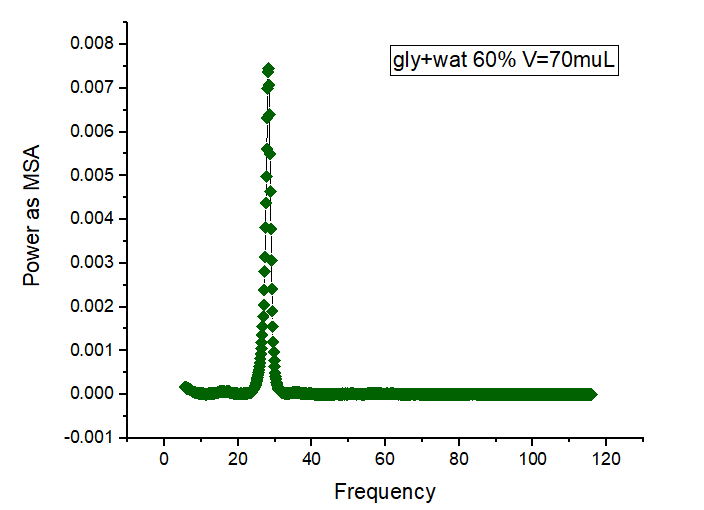
\includegraphics[width=.45\columnwidth]{gly_60.PNG}
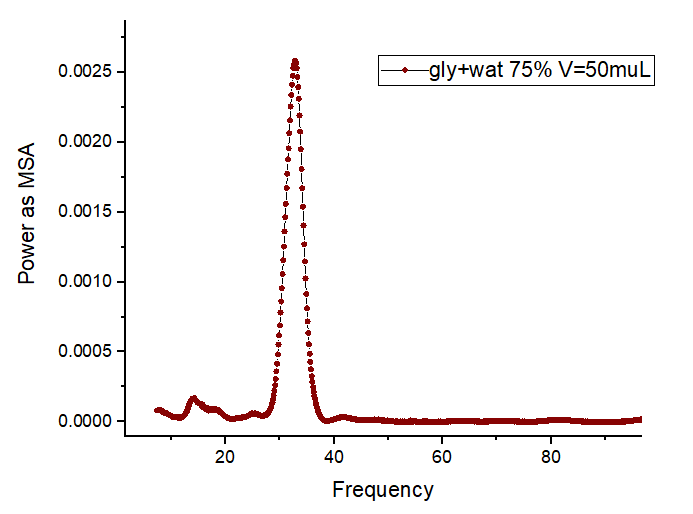
\includegraphics[width=.45\columnwidth]{gly_75.PNG}\\
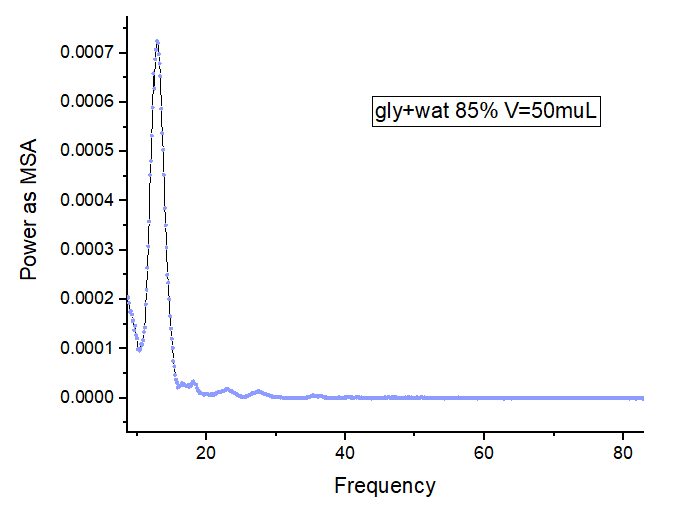
\includegraphics[width=.45\columnwidth]{gly_85.PNG}
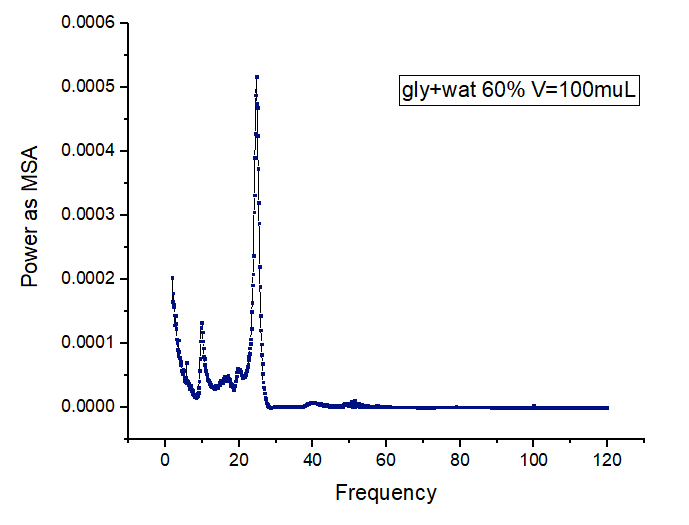
\includegraphics[width=.45\columnwidth]{gly_segnale_sporco.PNG}\\

\end{frame}

%%%%%%%%%%%%%%%%%%%%%%%%%%%%%%%%%%%%%%%%%%%%%%%%%%%%%%%%%%%%%%%%%%%

\begin{frame}

\frametitle{glycerol+water results}
\fontsize{10}{10.2} \selectfont
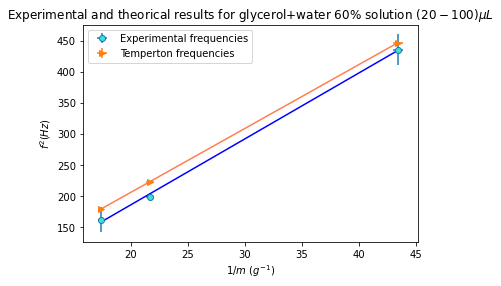
\includegraphics[width=.55\columnwidth]{grap_gly60.PNG}
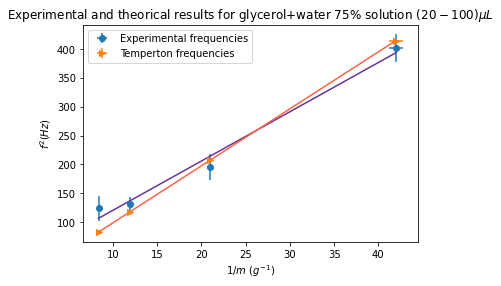
\includegraphics[width=.55\columnwidth]{grap_gly75.PNG}\\
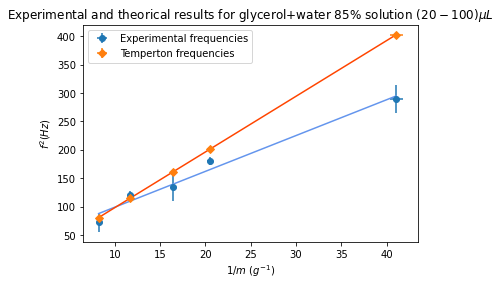
\includegraphics[width=.55\columnwidth]{grap_gly85.PNG}
\includegraphics[width=.45\columnwidth]{grap_gly85sc.PNG}\\

\end{frame}
%%%%%%%%%%%%%%%%%%%%%%%%%%%%%%%%%%%%%%%%%%%%%%%%%%%%%%%%%%%%%%%%%
\begin{frame}
\frametitle{Results - \textit{surface tension}}
\fontsize{9}{10.2} \selectfont
Used formula: 
\begin{equation}
 	\sigma=(2\pi)^2 F^2_n \frac{4\rho V}{\pi n^2} \frac{1}{tanh\bigg[\frac{n\pi}{4\theta}\frac{-cos^4\theta+6cos^2\theta-8cos\theta+3}{cos^3\theta-3cos\theta+2}\bigg]}
\end{equation}
Results:
\begin{table}[]
	\begin{tabular}{|c|c|c|c|}
		\hline
		(mN/m)   & Literature*     & Experimental (Pendant Drop) & \begin{tabular}[c]{@{}l@{}}Experimental (using\\ experimental frequencies)\end{tabular} \\
		\hline
		Acqua UP & $\simeq 72$ & $72,2 \pm 0,3$              & $73 \pm 1$                                                                                      \\
		gly 60\% & $\simeq 67$ & $66,9 \pm 0,5$              & $70 \pm 2$                                                                                      \\
		gly 75\% & $\simeq 65$ & $64 \pm 0,6$                & $67 \pm 2$                                                                                      \\
		gly 85\% & $\simeq 63$ & $63 \pm 1$                  & $59 \pm 3$              \\
		\hline                                                                       
	\end{tabular}
\end{table}
*da \textit{Physical properties of glycerine and its solutions} - C. S. Miner and N. N. Dalton.
\end{frame}

%%%%%%%%%%%%%%%%%%%%%%%%%%%%%%%%%%%%%%%%%%%%%%%%%%%%%%%%%%%%%%%%%%%

\begin{frame}

\frametitle{Results - \textit{viscosity}}
\fontsize{11}{10.2} \selectfont
Used formula:
\begin{equation}
	 \eta = \frac{\Gamma_{bulk}}{\frac{2}{\rho}\big(\frac{n\pi}{L}\big)^2}, \ \ \ \ with\ \Gamma_{bulk} =FWHM
\end{equation}
Results:
\begin{table}[]
	\begin{tabular}{|c|c|c|}
		\hline
		(mPa/s)  & Literature*  (T=$30^\circ$) & Experimental  \\ 
		\hline
		Acqua UP & $\simeq 1$ & $1,25 \pm 0,02$ \\
		gly 60\% & $\simeq 7,19$ & $7,3 \pm 0,1$     \\
		gly 75\% & $\simeq 21,2$ & $22,4 \pm 0,4$   \\
		gly 85\% & $\simeq 58$  & $52,6 \pm 0,3$\\
	\hline  
	\end{tabular}
\end{table}
\fontsize{9}{10.2} \selectfont
*da \textit{Physical properties of glycerine and its solutions} - C. S. Miner and N. N. Dalton.
\end{frame}

%%%%%%%%%%%%%%%%%%%%%%%%%%%%%%%%%%%%%%%%%%%%%%%%%%%%%%%%%%%%%%%%%%%

\begin{frame}

\frametitle{Graphics -Water}
\fontsize{10}{10.2} \selectfont
\includegraphics[width=0.8\columnwidth]{grafvisc.PNG}
\end{frame}

\begin{frame}

\frametitle{Graphics - Glycerol solutions}

\fontsize{10}{10.2} \selectfont
\centering
\includegraphics[width=0.5\columnwidth]{glyvisc.PNG}\\
\begin{columns}
	\begin{column}{.5\textwidth}
\includegraphics[width=0.9\columnwidth]{multipeaks.PNG}
\end{column}
	\begin{column}{.6\textwidth}
\includegraphics[width=0.8\columnwidth]{FWHM.PNG}
\end{column}
\end{columns}
\end{frame}
%%%%%%%%%%%%%%%%%%%%%%%%%%%%%%%%%%%%%%%%%%%%%%%%%%%%%%%%%%%%%%%%%%%

\begin{frame}

\frametitle{Conclusions}
\fontsize{11}{10.2} \selectfont

In this research activity I studied rheological properties of some type of Newtonian fluids.\\
\medskip
Problems that I found:
\begin{itemize}
	\item Uncontrolled gas puff
	\item Lack of data for some volumes
	\item Peak shape not always proper for data analyzing
	
\end{itemize}
\medskip 
Possible solutions:
\begin{itemize}
	\item To get a gas diffuser to be controlled remotely by an electrovalve
	\item Increase the statistics and create better ambiental conditions
	\item Program a software to control better the fitting parameters and improve the signal
\end{itemize}
\medskip
Once the apparatus will be optimized,  it will be possible to proceed to analize non-newtonian fluids.
\end{frame}
%%%%%%%%%%%%%%%%%%%%%%%%%%%%%%%%%%%%%%%%%%%%%%%%%%%%%%%%%%%%%%%%%

\end{document}